\documentclass[10pt,journal]{IEEEtran}
\usepackage[T1]{fontenc}
\usepackage{cite}
\usepackage{amsmath,amssymb,amsfonts}
\usepackage{graphicx}
\usepackage{algorithm}
\usepackage{algorithmic}
\usepackage[table]{xcolor}
\usepackage{url}
\usepackage{booktabs}
\usepackage{multirow}
\usepackage{adjustbox}
% ---------- Main comparison table style ----------
\usepackage{makecell}
\usepackage{array}

% Ranking fills: desaturated slate, print-safe and distinct in grayscale.
\definecolor{tblbest}{RGB}{186,206,219}
\definecolor{tblsecond}{RGB}{226,234,239}
\definecolor{abfull}{gray}{0.90} % light-gray highlight row for SOAR (Full) in ablation tables

\newcommand{\best}[1]{\cellcolor{tblbest}\textbf{#1}}
\newcommand{\second}[1]{\cellcolor{tblsecond}{#1}}
\newcommand{\na}{--}

\begin{document}
\title{Beyond Band Importance: Signed Orientation-Aware Spectral Learning for Graph Fraud Detection}
\author{Chunwei Tian, \emph{Senior Member, IEEE},
Qi Meng, \emph{Student Member, IEEE},
\thanks{This work was supported in part by xxx. (\textit{Corresponding authors: Chunwei Tian.})}%
\thanks{Chunwei Tian is with the School of Computer Science and Technology, Harbin Institute of Technology, Harbin 150001, China (e-mail: chunweitian@hit.edu.cn).}%
\thanks{Qi Meng is with the School of Computing and Data Science, The University of Hong Kong, Hong Kong, China (e-mail: kim.mengqi@connect.hku.hk).}%
}
\markboth{IEEE Transactions on Knowledge and Data Engineering}%
{Author \MakeLowercase{\textit{et al.}}: Not All Bands Are Neutral: Signed Orientation-Aware Residual for Graph Fraud Detection}

\IEEEtitleabstractindextext{
\begin{abstract}
Spectral graph neural networks have shown strong potential for fraud detection by capturing graph signals across different frequency bands. However, existing spectral approaches mainly assess which bands are informative, while paying less attention to which class each band favors. Consequently, spectral responses supporting fraud and benign classes may be blended during representation learning, especially when limited supervision makes such class orientations difficult to estimate reliably. To address this issue, we propose Signed Orientation-Aware Residual (SOAR), a spectral framework that explicitly preserves class-oriented evidence at the relation--band level. SOAR infers the class orientation of spectral responses from relation-specific energy patterns and available labels, while estimating how reliable these orientations are across relations. It then preserves reliable orientation cues through signed residual learning, while retaining orientation-neutral spectral information when the estimated directions are uncertain. A directional consistency objective further regularizes the learned representations toward the inferred class orientations. Experiments on four public fraud graphs under both abundant and scarce supervision show that SOAR consistently improves over strong spectral baselines, with particularly clear gains on multi-relation graphs where relation-dependent spectral orientations are more pronounced. Code is available at \url{[https://github.com/xxx/SOAR}].

\end{abstract}
\begin{IEEEkeywords}
Graph fraud detection, graph neural networks, heterophily, spectral graph learning.
\end{IEEEkeywords}}
\maketitle
\IEEEdisplaynontitleabstractindextext

\section{Introduction}
\label{sec:introduction}

\IEEEPARstart{O}{nline} banking, e-commerce, and social platforms are increasingly threatened by organized fraud. Malicious accounts often coordinate to conduct fraudulent transactions, manipulate reviews, and engage in other forms of collective abuse \cite{cheng2025fraudreview}. Graph-based fraud detection exploits relational structures among entities to uncover such coordinated patterns, which are difficult to identify from node attributes alone \cite{ma2023gadsurvey}. However, fraudsters often evade detection by mimicking benign attributes while deliberately connecting to legitimate entities, causing fraud graphs to exhibit feature homophily and label heterophily simultaneously \cite{zheng2026heterophily}. Consequently, homophilic and heterophilic signals coexist within local neighborhoods, where different neighbors may provide evidence favoring opposite classes. Conventional neighborhood aggregation can therefore blur conflicting class evidence into a single representation, making reliable fraud detection particularly challenging.

\begin{figure}[!t]
\centering
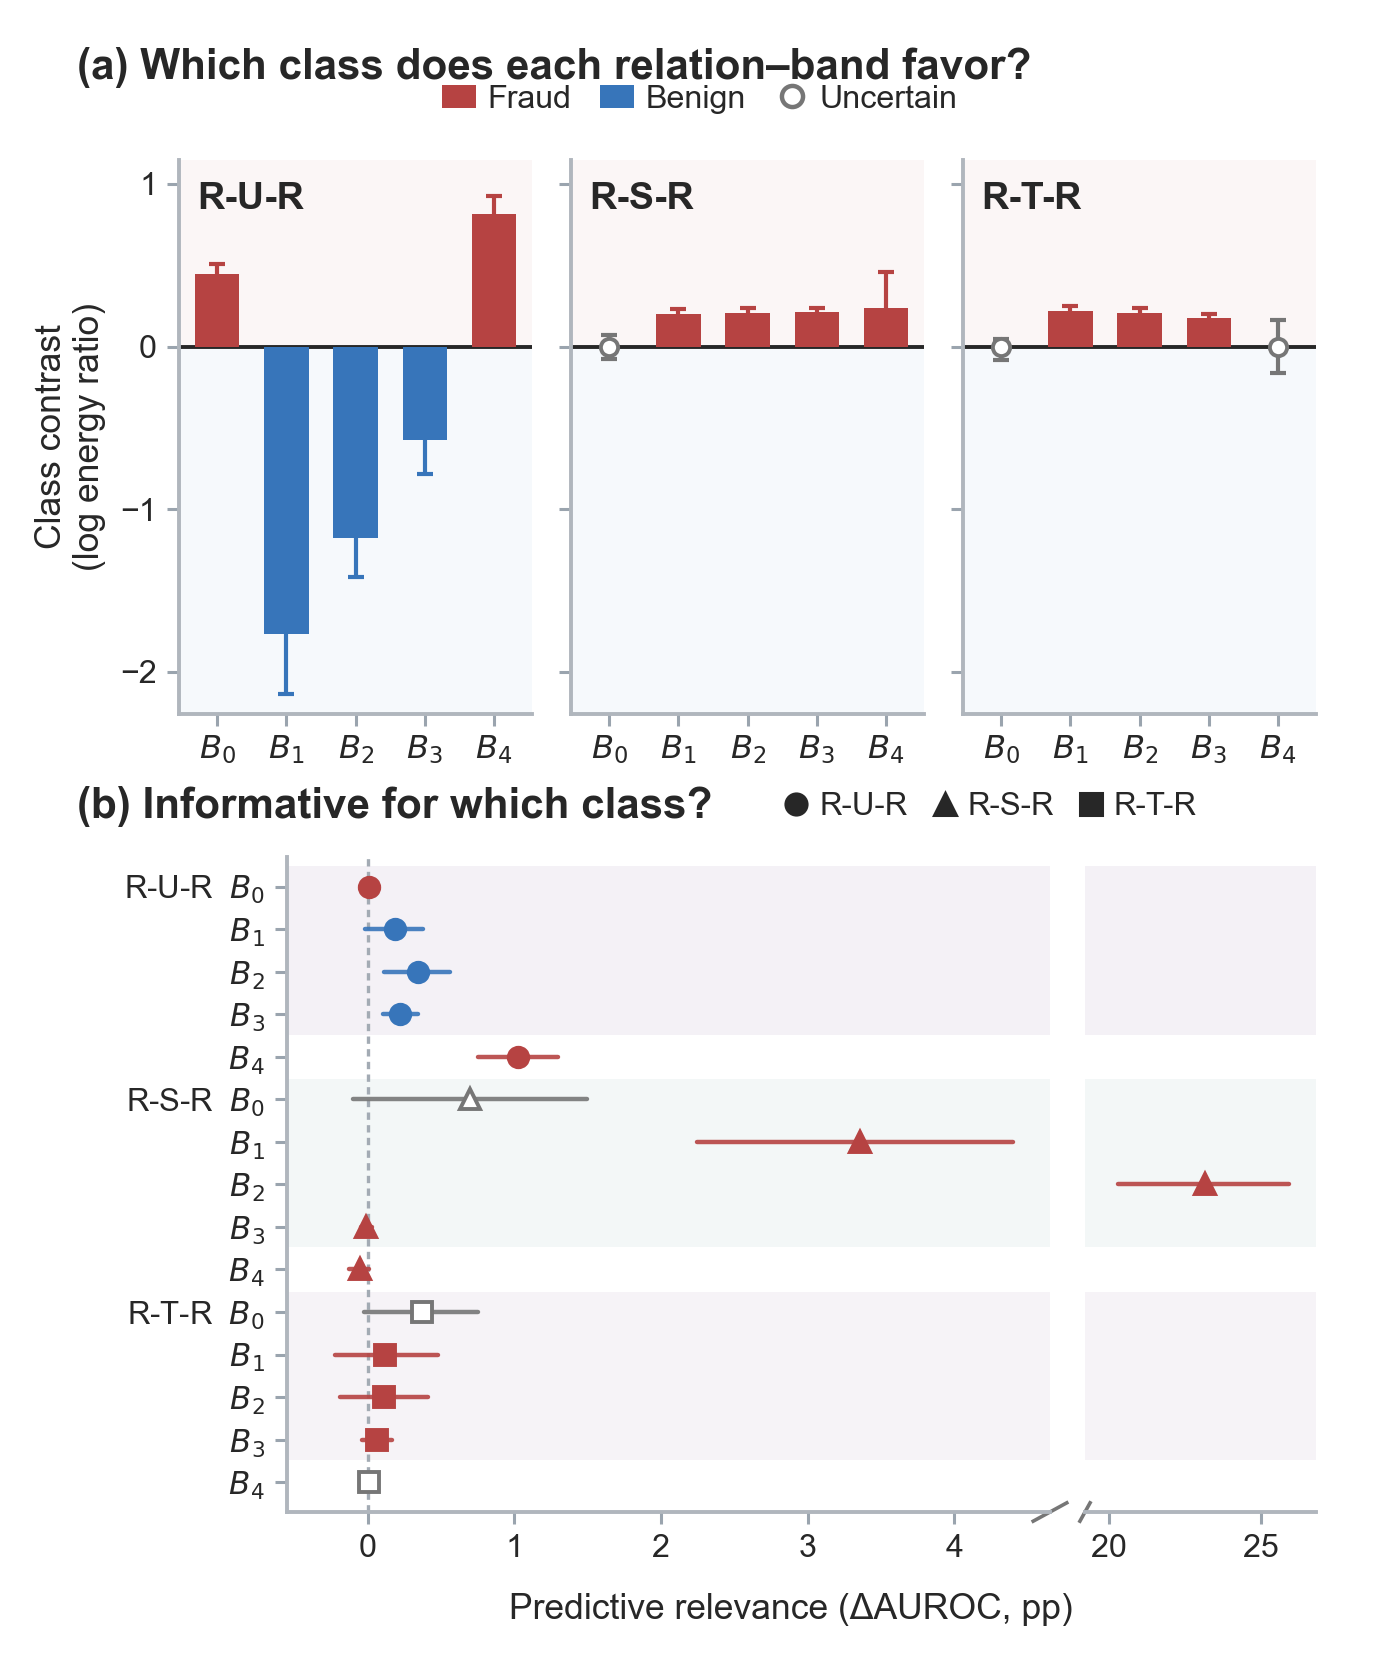
\includegraphics[width=0.8\columnwidth]{fig_motivation.png}
\caption{Beyond band importance: empirical motivation on YelpChi. Using a shared Beta-wavelet bank, we examine (a)~class-conditional band-response energy and (b)~predictive relevance versus class orientation. Positive relevance appears on both sides of the class boundary, so band importance does not specify which class a relation--band supports.}
\label{fig:motivation}
\end{figure}

\begin{figure*}[!t]
\centering
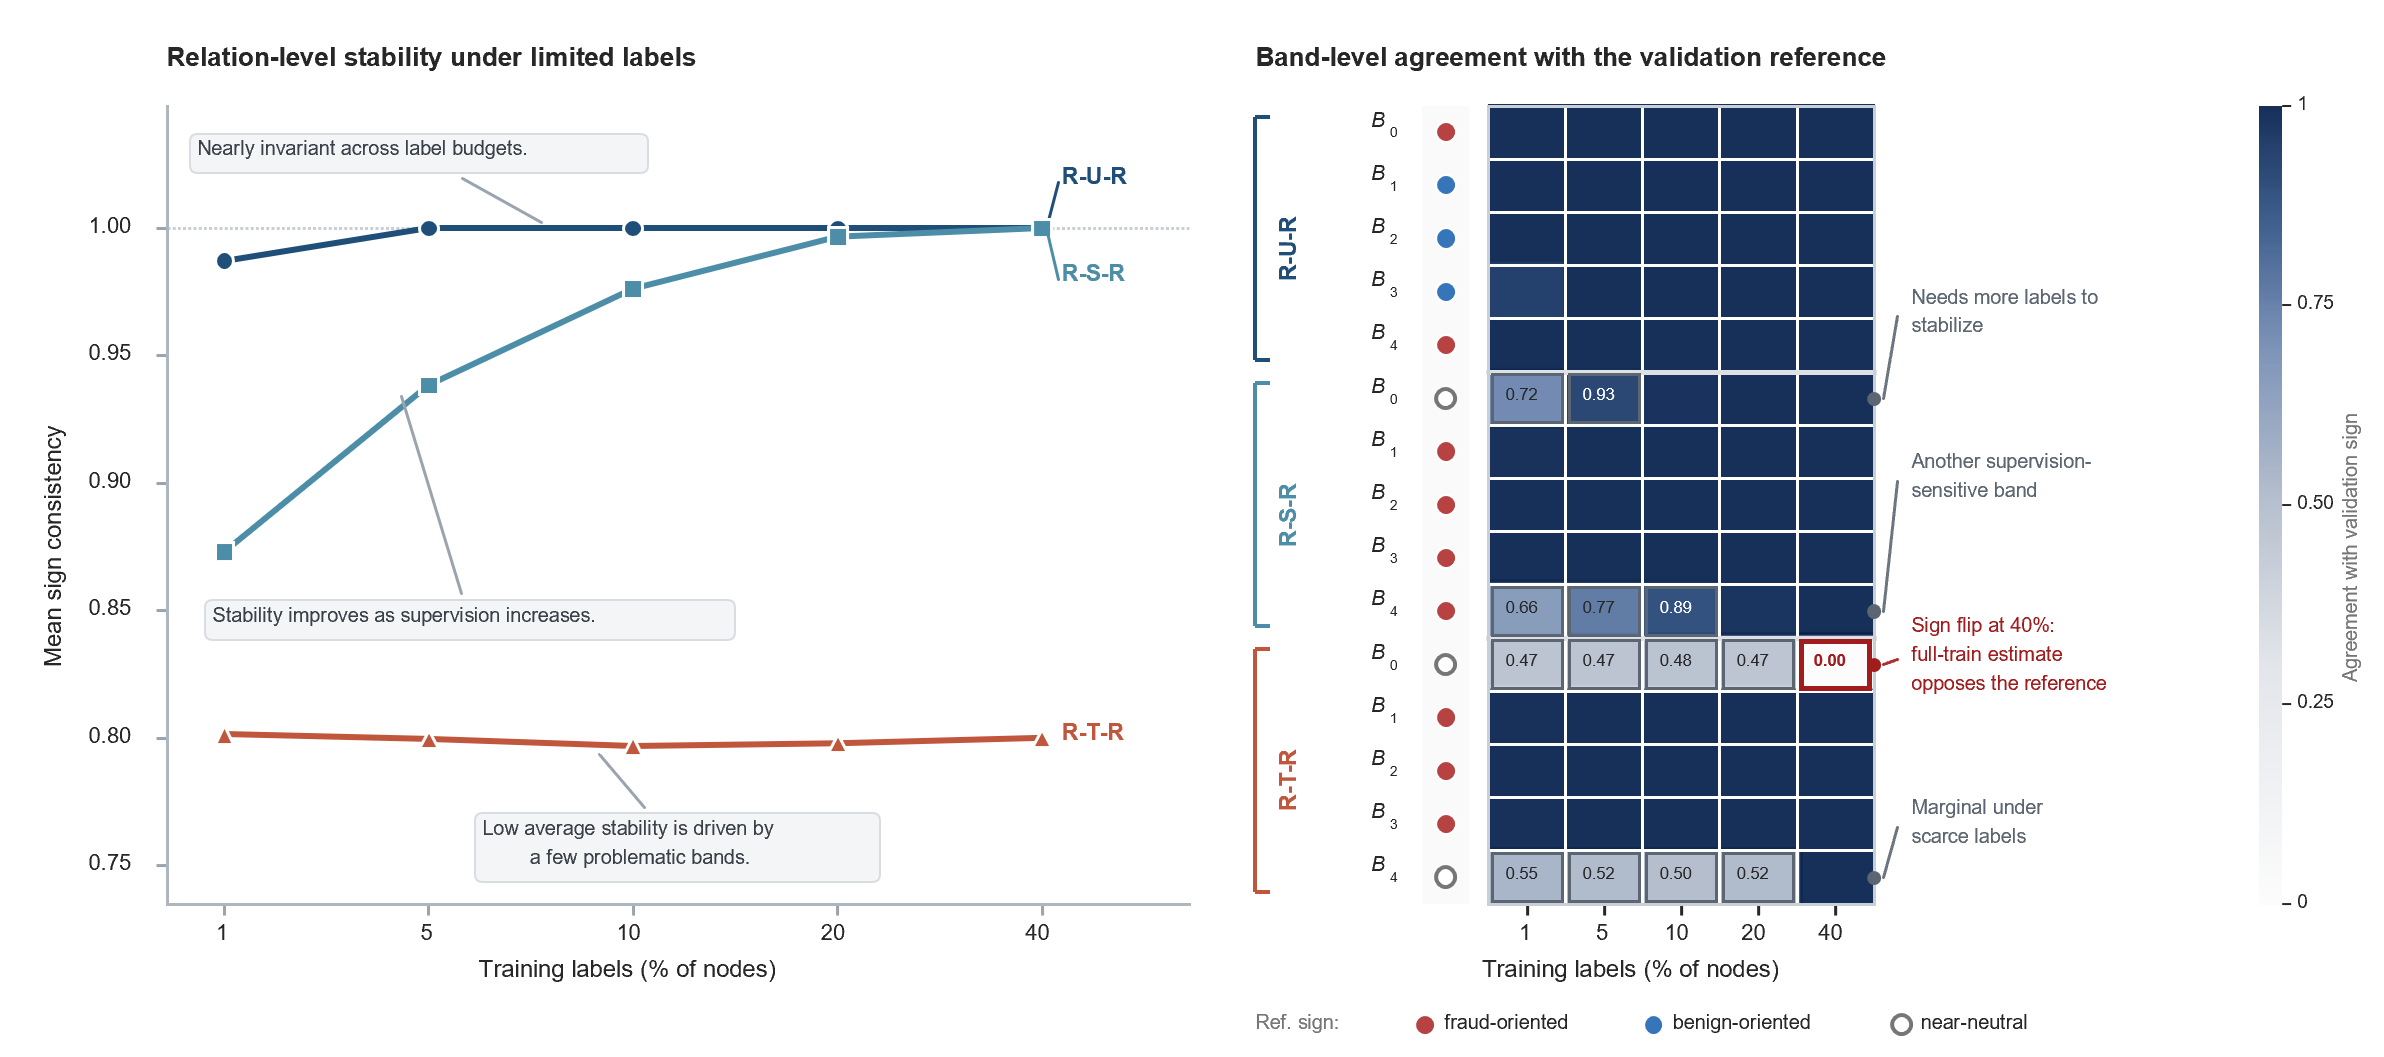
\includegraphics[width=0.8\textwidth]{fig_reliability.png}
\caption{Direction estimates are not equally reliable on YelpChi. Stability is the proportion of 1{,}000 stratified draws from the training pool whose estimated signs agree with the validation reference. Left: relation-level averages. R-U-R remains stable even under scarce labels, R-S-R becomes stable as supervision increases, and R-T-R stays markedly less reliable. Right: band-level agreement with the validation reference. R-S-R $B_0$ and $B_4$ require more labels to stabilize, whereas R-T-R $B_0$ is persistently unreliable and even flips against the validation reference when the full training pool is used.}
\label{fig:reliability}
\end{figure*}

Existing methods address this challenge mainly from spatial and spectral perspectives. Generic graph neural networks, such as GCN \cite{kipf2017gcn} and GAT \cite{velickovic2018gat}, encode local connectivity through neighborhood aggregation, but may indiscriminately combine signals with different class orientations when homophily and heterophily coexist. Spatial fraud detectors, including CARE-GNN \cite{dou2020caregnn}, PC-GNN \cite{liu2021pcgnn}, and H2-FDetector \cite{shi2022h2fdetector}, mitigate this issue through neighbor filtering, relation modeling, or heterophily-aware aggregation, yet their primary focus remains local node interactions. Spectral approaches instead characterize graph structure through frequency responses \cite{shuman2013emerging}. BWGNN \cite{tang2022bwgnn}, AMNet \cite{chai2022amnet}, and SplitGNN \cite{wu2023splitgnn} exploit multi-band decomposition and frequency selection to capture informative spectral patterns, while GHRN \cite{gao2023ghrn} and EOGFD \cite{wang2026eogfd} further adapt spectral responses using heterophily or topological information. Despite these advances, existing spectral methods primarily focus on determining which frequencies are informative, rather than which class their responses support.

This distinction is crucial because frequency importance does not imply class orientation (Fig.~\ref{fig:motivation}). Within the same relation, different frequency bands may provide evidence favoring the fraud and benign classes, respectively. If such orientation is not modeled explicitly, responses that are individually informative but favor opposite classes may be blended during representation learning, weakening the resulting class evidence. The problem becomes more pronounced under limited supervision, where the reliability of orientation estimates can vary substantially across relations (Fig.~\ref{fig:reliability}); enforcing uncertain orientations too strongly may introduce additional noise. Therefore, spectral fraud detection requires more than identifying informative frequencies: it must also determine which class each relation--band response favors and how much that orientation should be trusted.

To address this gap, we propose Signed Orientation-Aware Residual (SOAR), which explicitly models and preserves class-oriented spectral evidence at the relation--band level. SOAR first constructs relation--band energy representations from observed node attributes and uses training labels to estimate the class orientation of each relation--band response. It further estimates relation-level reliability to quantify how strongly these orientations should influence prediction. The estimated orientations are then encoded as signed residuals and injected into their corresponding spectral bands, preserving class-oriented evidence throughout subsequent representation learning. To remain robust when orientation estimates are uncertain, SOAR adopts a dual-path prediction architecture. The orientation-aware path modulates signed residuals according to relation-level reliability, emphasizing trustworthy directional evidence, while an orientation-neutral spectral path retains spectral information without committing to a particular class orientation. In addition, an orientation-consistency constraint encourages the learned discriminative representations to remain aligned with the estimated orientations.

The main contributions of this work are summarized as follows:

\begin{itemize}
\item
We characterize spectral responses from the perspective of class orientation, explicitly distinguishing evidence that favors fraud from evidence that favors the benign class, thereby preventing oppositely oriented responses from being indiscriminately mixed in subsequent representations.

\item 
We jointly model relation--band orientations and relation-level reliability, allowing directional evidence to be adaptively weighted under limited supervision and reducing the influence of unreliable orientation estimates on prediction.

\item 
We combine a dual-path predictor with an orientation-consistency constraint to exploit reliable class-oriented evidence while retaining orientation-neutral spectral information when orientation estimates are uncertain.

\end{itemize}
The remainder of this paper is organized as follows.
Section~\ref{sec:related_work} reviews related work on graph fraud detection.
Section~\ref{sec:method} formulates the detection problem and presents the proposed SOAR framework.
Section~\ref{sec:experiments} reports the experimental results and analysis.
Finally, Section~\ref{sec:conclusion} concludes the paper.

\section{Related Work}
\label{sec:related_work}

\subsection{Spatial Graph Learning for Fraud Detection}

Graph fraud detection leverages interactions among entities connected through transactions, reviews, followings, and other behavioral links \cite{cheng2025fraudreview}. Because fraudsters often mimic benign users and deliberately connect to legitimate entities, local neighborhoods may contain both informative and misleading interactions. Spatial methods have therefore developed mainly along two directions: refining the quality of local interactions and adapting message passing to mixed homophilic and heterophilic structures.

Along the first direction, CARE-GNN \cite{dou2020caregnn} performs relation-specific neighbor filtering based on feature similarity, PC-GNN \cite{liu2021pcgnn} introduces label-aware sampling to alleviate class imbalance, and GraphConsis \cite{liu2020graphconsis} learns consistency-aware weights for noisy multi-relation interactions. Later methods incorporate additional feature or structural cues, such as discriminative interaction modeling in DiG-In-GNN \cite{zhang2024digingnn} and community structure in CMRGNN \cite{han2025cmrgnn}. Although these methods assess local interactions in different ways, they share the goal of suppressing unreliable messages before aggregation. This improves robustness to camouflage, but interaction reliability and class orientation describe different properties of the signal: even informative interactions may provide evidence favoring different classes.

A complementary direction models homophilic and heterophilic interactions more explicitly. Fraud-specific methods such as H2-FDetector \cite{shi2022h2fdetector}, H2IDE \cite{fu2025h2ide}, and DHMP \cite{zhang2025dhmp} separate or adapt different types of local signals through heterophily-aware aggregation, disentangled representations, or multi-channel propagation. Related principles also appear in general heterophilic graph learning. H2GCN \cite{zhu2020h2gcn}, FAGCN \cite{bo2021fagcn}, and GloGNN \cite{li2022glognn} modify propagation or representation coupling to better accommodate heterophilic structure, while LINKX \cite{lim2021linkx} and graph rewiring \cite{bi2024rewiring} reduce dependence on standard neighborhood aggregation through feature--topology decoupling or structural adjustment. Other approaches incorporate class or homophily cues more directly: CPGNN \cite{zhu2021cpgnn} exploits class compatibility, GAGA \cite{wang2023gaga} introduces label-aware group aggregation, RHO \cite{ai2025rho} combines heterogeneous homophily with adaptive frequency responses, and HUGE \cite{pan2025huge} estimates heterophilic structure without relying directly on labels. Together, these studies substantially improve how information is selected and propagated under camouflage and heterophily. Their main modeling focus nevertheless remains on nodes, relations, or propagation patterns. Even when signed propagation or frequency-aware mechanisms are involved, these mechanisms primarily regulate information flow rather than explicitly associate a relation-specific frequency response with the class it favors. This motivates a finer-grained view in which class orientation is examined jointly across relations and frequency bands.

\subsection{Spectral Graph Learning for Fraud Detection}

Spectral graph learning \cite{shuman2013emerging,ortega2018gsp} represents graph signals through frequency responses and provides a natural view of structural variation across different scales. Early graph wavelets \cite{hammond2011wavelets} and spectral convolution \cite{bruna2014spectral} established the foundations of frequency-domain graph filtering. ChebNet \cite{defferrard2016chebnet} introduced localized polynomial filtering, while GCN \cite{kipf2017gcn} simplified spectral propagation through a first-order approximation. Later architectures improved filter flexibility: GPR-GNN \cite{chien2021gprgnn} learns positive and negative coefficients over different propagation orders, whereas ChebNetII \cite{he2022chebnetii} reparameterizes Chebyshev filters to obtain more expressive responses. These models demonstrate that adaptive or signed coefficients can effectively control how propagation components contribute to a representation. Importantly, the sign of such a coefficient is primarily an algebraic property of the filtering process and does not necessarily correspond to the class favored by the resulting response. This distinction is particularly relevant to fraud detection, where frequency bands of comparable predictive value may support different classes.

Building on these filtering principles, spectral fraud detectors exploit multi-band structure to capture anomalous and camouflaged behavior. BWGNN \cite{tang2022bwgnn} models anomalies across multiple spectral scales using Beta wavelet filters, while AMNet \cite{chai2022amnet} learns adaptive spectral responses to emphasize informative frequency components. Several methods further incorporate heterophily or local structural information: GHRN \cite{gao2023ghrn} relates heterophily to high-frequency signals, SplitGNN \cite{wu2023splitgnn} combines edge separation with band-pass filtering, and SEC-GFD \cite{xu2024secgfd} models mixed-frequency responses under local structural constraints. A parallel line improves spectral adaptation across nodes, neighborhoods, or graph dynamics. F-GNN \cite{zhao2026fgnn} learns node-adaptive filters, NAAST \cite{guo2024naast} couples neighborhood adaptation with spectral tuning, DSGAD \cite{zheng2025dsgad} adapts spectral representations to evolving graphs, DPF \cite{he2026dpf} employs dual-path filtering to capture complementary response patterns, and EGNN \cite{liu2026egnn} models left- and right-shift spectral energy in static and temporal graphs. Collectively, these studies have substantially advanced frequency decomposition, selection, and adaptation for fraud detection.

Despite these advances, existing spectral fraud detectors mainly focus on identifying informative frequencies and adapting their contributions to graph structure, while the class orientation of relation-specific band responses remain less explored. Different bands within the same relation may be similarly predictive yet favor opposite classes, and such distinctions can be blurred when their responses are combined. Under limited supervision, their inferred orientations may also vary in reliability across relations. SOAR addresses these issues by jointly modeling relation--band class orientation and relation-level reliability, while preserving orientation-neutral spectral information when the estimated orientation is uncertain. Building on this perspective, Section~\ref{sec:method} first formalizes the problem setting and relation-wise spectral decomposition, and then develops SOAR around class orientation and relation-level reliability.

\section{Proposed Method}
\label{sec:method}

\subsection{Problem Definition}
\label{sec:problem}

Given an attributed multi-relation graph
$\mathcal{G}=(\mathcal{V},\{\mathcal{E}_r\}_{r=1}^{R},\mathbf{X})$,
$\mathcal{V}=\{v_1,\ldots,v_N\}$ denotes the set of $N$ nodes,
$\mathcal{E}_r$ denotes the edge set associated with relation $r$, and
$\mathbf{X}\in\mathbb{R}^{N\times d}$ is the node-feature matrix, where
$\mathbf{x}_i\in\mathbb{R}^{d}$ represents the attributes of node $v_i$.
Each relation is represented by a symmetric nonnegative adjacency matrix
$\mathbf{A}_r\in\mathbb{R}^{N\times N}$.
Only a subset of nodes
$\mathcal{V}_{\mathrm L}\subset\mathcal{V}$ is labeled for training, with
$y_i\in\{0,1\}$, where $y_i=1$ denotes fraud and $y_i=0$ denotes a benign node.
The remaining nodes
$\mathcal{V}_{\mathrm U}=\mathcal{V}\setminus\mathcal{V}_{\mathrm L}$
are unlabeled during training.
We consider the transductive setting, where graph structure and node
attributes are observable for all nodes, while training supervision is
restricted to $\mathcal{V}_{\mathrm L}$.
The goal is to learn a predictor
$F_{\Theta}:\mathcal{V}\rightarrow[0,1]$
that estimates the fraud probability of each node, where $\Theta$ denotes
the collection of learnable model parameters.

Our focus is on the spectral evidence underlying this prediction.
In multi-relation fraud graphs, frequency bands within and across relations
may exhibit distinct, and potentially opposing, class preferences, while
limited supervision provides uneven support for identifying these preferences.
The central challenge is therefore to exploit such class-oriented spectral
differences without allowing uncertain or conflicting evidence to dominate
prediction.


\subsection{Overview}
\label{sec:overview}

SOAR is designed to model class-oriented spectral evidence in multi-relation
fraud graphs. As illustrated in Fig.~\ref{fig:framework}, it consists of three
main modeling components: orientation estimation, in-band signed residual
construction, and dual-path prediction. The orientation estimator identifies
which class each relation--band response favors and evaluates the reliability
of these orientations at the relation level. The in-band signed residual
injects each estimated orientation into its corresponding hidden spectral
band, while the dual-path predictor combines the resulting orientation-aware
residual with orientation-neutral spectral information. A directional-consistency
objective further regularizes the learned representations during training.
The following subsections detail these components and the training objective.

\begin{figure*}[!t]
    \centering
    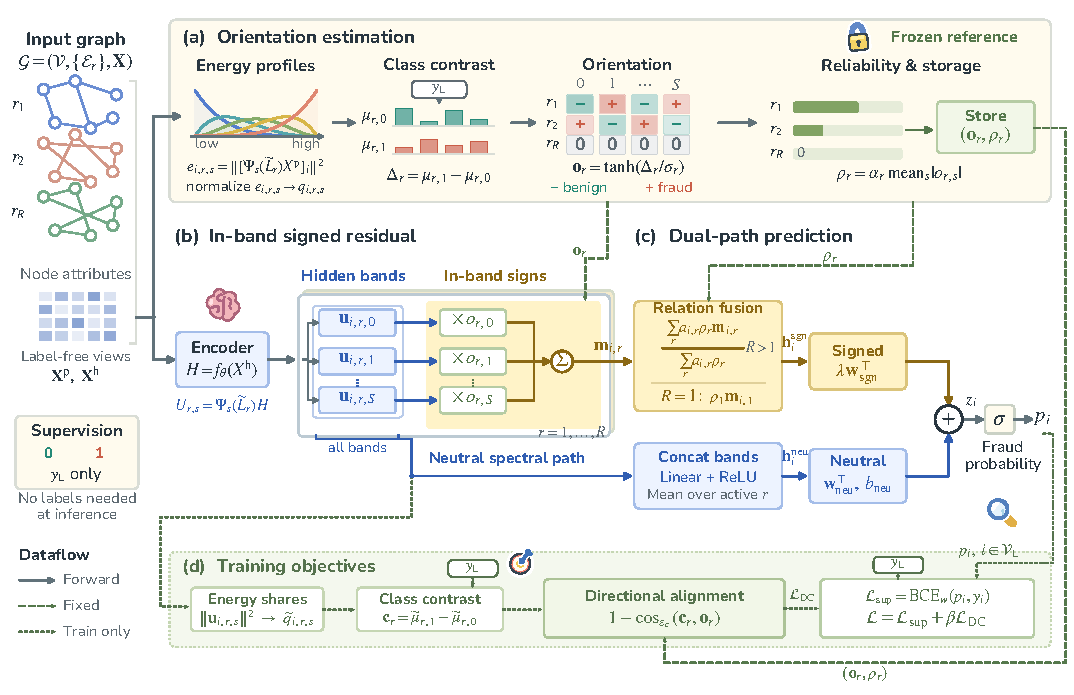
\includegraphics[width=\textwidth]{fig_framework.pdf}
    \caption{Overview of SOAR.
(a) Observed-feature spectral profiles and training labels yield fixed
relation--band orientations $\mathbf{o}_r$ and relation reliabilities $\rho_r$.
Reliability combines balanced training support and orientation strength.
(b) The same spectral bank produces hidden responses; each $o_{r,s}$ acts on
its matching band before band summation and reliability-aware relation fusion.
Single-relation fusion retains absolute reliability scaling.
(c) An orientation-neutral path uses the raw hidden bands, independently of
$\mathbf{o}_r$ and $\rho_r$. Its logit and the bias-free signed contribution
are added before the sigmoid.
(d) During training, reliability-weighted cosine alignment regularizes hidden
class contrasts toward the fixed orientations, jointly with weighted binary
cross-entropy. The consistency gate requires both signs collectively among
targets with $\rho_r>0$; empty targets or an inactive gate give zero loss.
Unsupported multi-relation signed fusion also returns zero.
The reference estimator remains outside optimization; inference requires no labels.
Dashed arrows carry fixed references; dotted arrows denote training-only
computations. Miniature graphs, profiles, and sign patterns are schematic.}
    \label{fig:framework}
\end{figure*}

\subsection{Orientation Estimation}
\label{sec:orientation}

The first component of SOAR estimates the class orientation of each
relation--band response together with relation-level reliability. Both
quantities are derived from observed node features and the available training
labels before model optimization, providing a fixed spectral reference for
subsequent representation learning.

\paragraph{Relation--band energy profiles}
For relation $r$, let $\mathbf{D}_r$ denote the diagonal degree matrix of
$\mathbf{A}_r$. We define the normalized graph Laplacian as
\begin{equation}
\widetilde{\mathbf{L}}_r
=
\mathbf{I}
-
\mathbf{D}_r^{-1/2}
\mathbf{A}_r
\mathbf{D}_r^{-1/2},
\label{eq:laplacian}
\end{equation}
where $\mathbf{I}\in\mathbb{R}^{N\times N}$ is the identity matrix and
inverse degrees are set to zero for isolated nodes.

Let
$d_{i,r}=[\mathbf{D}_r]_{ii}$
denote the degree of node $i$ under relation $r$, and define
\begin{equation}
a_{i,r}
=
\mathbb{I}[d_{i,r}>0],
\label{eq:active}
\end{equation}
where $\mathbb{I}[\cdot]$ denotes the indicator function.

Since the spectrum of $\widetilde{\mathbf{L}}_r$ lies in $[0,2]$, we employ
a bank of $K=S+1$ Bernstein polynomial filters of order $S$,
\begin{equation}
\Psi_s(\widetilde{\mathbf{L}}_r)
=
\binom{S}{s}
\left(\frac{\widetilde{\mathbf{L}}_r}{2}\right)^s
\left(
\mathbf{I}
-
\frac{\widetilde{\mathbf{L}}_r}{2}
\right)^{S-s},
\qquad
s=0,\ldots,S,
\label{eq:bernstein}
\end{equation}
which provide overlapping responses from low to high graph frequencies
\cite{shuman2013emerging,tang2022bwgnn}.

Let $\mathbf{X}^{\mathrm p}$ denote the label-free feature input derived from
$\mathbf{X}$ for orientation profiling. For a node active under relation $r$,
its response energy in band $s$ and the corresponding normalized energy share
are
\begin{equation}
\begin{aligned}
e_{i,r,s}
&=
\left\|
\left[
\Psi_s(\widetilde{\mathbf{L}}_r)
\mathbf{X}^{\mathrm p}
\right]_{i,:}
\right\|_2^2,\\
q_{i,r,s}
&=
\frac{e_{i,r,s}}
{\max\left\{
\sum_{t=0}^{S}e_{i,r,t},
\varepsilon_e
\right\}},
\end{aligned}
\label{eq:profile}
\end{equation}
where $\varepsilon_e>0$ is a small constant for numerical stability.
We collect the normalized band responses as
\begin{equation}
\mathbf{q}_{i,r}
=
[q_{i,r,0},\ldots,q_{i,r,S}]^\top
\in\mathbb{R}^{K}.
\label{eq:profile_vector}
\end{equation}
The squared norm summarizes response strength across feature dimensions,
whereas the node-wise normalization removes the overall response scale and
retains the relative allocation of energy across bands. Thus,
$\mathbf{q}_{i,r}$ describes the spectral distribution of the observed
attributes under relation $r$ without using label information.

\paragraph{Class orientation}
The labeled support of class $c\in\{0,1\}$ under relation $r$ is
\begin{equation}
\mathcal{V}_{r,c}
=
\left\{
i\in\mathcal{V}_{\mathrm L}
\,\middle|\,
a_{i,r}=1,\; y_i=c
\right\},
\qquad
n_{r,c}=|\mathcal{V}_{r,c}|.
\label{eq:relation_support}
\end{equation}
A relation is considered resolved only when
$n_{r,0}\ge2$ and $n_{r,1}\ge2$.
Otherwise, its orientation and reliability are set to zero.
For a resolved relation, we compute the class-conditional mean profile
\begin{equation}
\boldsymbol{\mu}_{r,c}
=
\frac{1}{n_{r,c}}
\sum_{i\in\mathcal{V}_{r,c}}
\mathbf{q}_{i,r},
\label{eq:class_profile}
\end{equation}
and define the fraud-minus-benign spectral contrast as
\begin{equation}
\boldsymbol{\Delta}_r
=
\boldsymbol{\mu}_{r,1}
-
\boldsymbol{\mu}_{r,0}.
\label{eq:class_contrast}
\end{equation}
Accordingly, a positive $\Delta_{r,s}$ indicates that fraud nodes allocate
relatively more energy to band $s$, whereas a negative value indicates the
opposite.

Because the natural dispersion of energy shares can differ across bands,
we compute the coordinate-wise sample deviation over the combined labeled
support,
\begin{equation}
\boldsymbol{\sigma}_r
=
\max\left\{
\operatorname{Std}_{\mathrm{sample}}
\left(
\left\{
\mathbf{q}_{i,r}
:
i\in
\mathcal{V}_{r,0}\cup\mathcal{V}_{r,1}
\right\}
\right),
\varepsilon_o
\right\},
\label{eq:orientation_scale}
\end{equation}
where $\varepsilon_o>0$ prevents degenerate scaling and the maximum is taken
coordinate-wise. The relation--band orientation is then defined as
\begin{equation}
\mathbf{o}_r
=
\tanh\left(
\frac{
\boldsymbol{\Delta}_r
}{
\boldsymbol{\sigma}_r
}
\right),
\label{eq:orientation}
\end{equation}
with all operations applied element-wise.

Each $o_{r,s}\in[-1,1]$ preserves the sign of the corresponding class contrast
while bounding its magnitude. Its sign indicates whether the relative energy
of band $s$ is larger for fraud or benign nodes, whereas $|o_{r,s}|$ reflects
the strength of this variance-normalized contrast. Importantly,
$o_{r,s}$ is a relation--band class reference rather than a node-level fraud
probability or a statistical significance score.

\paragraph{Relation-level reliability}
A pronounced orientation may still be unreliable when it is supported by
only a few labeled nodes from either class (Fig.~\ref{fig:reliability}). We therefore combine class support
with orientation strength. The balanced support of relation $r$ is measured by
\begin{equation}
n_r^{\mathrm{eff}}
=
\frac{2n_{r,0}n_{r,1}}
{n_{r,0}+n_{r,1}},
\qquad
\alpha_r
=
\min\left\{
\frac{n_r^{\mathrm{eff}}}{\tau_n},
1
\right\},
\label{eq:support_factor}
\end{equation}
where $n_r^{\mathrm{eff}}$ is the harmonic mean of the two class supports and
$\tau_n>0$ controls support saturation. The relation-level reliability is
then defined as
\begin{equation}
\rho_r
=
\alpha_r
\frac{1}{K}
\sum_{s=0}^{S}|o_{r,s}|.
\label{eq:reliability}
\end{equation}
Since both factors lie in $[0,1]$, $\rho_r\in[0,1]$.
A relation receives higher reliability when it has stronger labeled support
from both classes and, on average, more pronounced relation--band contrasts.
The quantity $\rho_r$ is a deterministic reliability weight rather than a
calibrated probability that an orientation is correct.

The resulting pair $(\mathbf{o}_r,\rho_r)$ is computed once using training
labels only and remains fixed throughout model optimization. This separates
the estimation of class-oriented spectral evidence from the learned
representation and prevents the orientation reference from adapting to the
downstream training objective.


\subsection{In-Band Signed Residual}
\label{sec:residual}

The estimated orientations in Section~\ref{sec:orientation} provide a fixed
class reference for individual relation--band responses. To preserve this
information during representation learning, SOAR injects each orientation
into its corresponding hidden band before different bands are aggregated.
This in-band operation prevents responses with opposite estimated orientations
from being treated identically in the learned representation.

Let $\mathbf{X}^{\mathrm h}$ denote the label-free feature input derived from
$\mathbf{X}$ for representation learning; it may coincide with
$\mathbf{X}^{\mathrm p}$. A learnable encoder $f_\theta$ maps the input
features to
\begin{equation}
\mathbf{H}
=
f_\theta(\mathbf{X}^{\mathrm h})
\in\mathbb{R}^{N\times d_h},
\label{eq:hidden}
\end{equation}
where $d_h$ is the hidden dimension and $\theta\subseteq\Theta$ denotes the
encoder parameters.

Using the same relation-wise spectral bank as in orientation estimation,
we obtain
\begin{equation}
\mathbf{U}_{r,s}
=
\Psi_s(\widetilde{\mathbf{L}}_r)\mathbf{H},
\qquad
r=1,\ldots,R,\;\;
s=0,\ldots,S.
\label{eq:hidden_band}
\end{equation}
For node $i$, let
\begin{equation}
\mathbf{u}_{i,r,s}
=
[\mathbf{U}_{r,s}]_{i,:}^{\top}
\in\mathbb{R}^{d_h}
\label{eq:hidden_band_node}
\end{equation}
denote its hidden response in band $s$ under relation $r$.

Rather than aggregating these responses without regard to their class
orientation, SOAR applies $o_{r,s}$ directly to its matching hidden band:
\begin{equation}
\mathbf{m}_{i,r}
=
\sum_{s=0}^{S}
o_{r,s}\mathbf{u}_{i,r,s}.
\label{eq:signed_mix}
\end{equation}
Equation~\eqref{eq:signed_mix} constitutes the \emph{in-band} signed
operation: the orientation estimated for $(r,s)$ acts only on the same
relation--band before cross-band aggregation. Its sign distinguishes opposing
class orientations, whereas its magnitude controls the contribution of the
corresponding band. This operation provides a representation-level orientation
prior rather than fixing the final class prediction, which remains determined
by the learned readout.

The relation-specific signed representations are further combined according
to relation-level reliability. For a multi-relation graph,
\begin{equation}
\mathbf{h}^{\mathrm{sgn}}_i
=
\frac{
\sum_{r=1}^{R}
a_{i,r}\rho_r\mathbf{m}_{i,r}
}{
\sum_{r=1}^{R}
a_{i,r}\rho_r
},
\qquad
R>1,
\label{eq:signed_fusion}
\end{equation}
whenever the denominator is positive; otherwise,
$\mathbf{h}^{\mathrm{sgn}}_i=\mathbf{0}$.
Here, $\rho_r$ serves as a relative weight among the relations available to
node $i$, allowing orientations supported by stronger evidence to contribute
more to the signed representation.

For a single-relation graph, the normalization in
Eq.~\eqref{eq:signed_fusion} would cancel the reliability term. We therefore
retain its absolute effect:
\begin{equation}
\mathbf{h}^{\mathrm{sgn}}_i
=
\rho_1\mathbf{m}_{i,1},
\qquad
R=1.
\label{eq:signed_single}
\end{equation}
The resulting $\mathbf{h}^{\mathrm{sgn}}_i$ forms the orientation-aware
residual used in prediction. It complements rather than replaces the
underlying spectral representation, motivating the dual-path design below.


\subsection{Dual-Path Prediction}
\label{sec:dual}

The signed residual preserves class-oriented spectral evidence, but its
orientation is inferred from limited supervision and may therefore be
uncertain for some relations. To avoid making prediction overly dependent
on directional estimates, SOAR retains the underlying spectral information
through a complementary orientation-neutral path.

\paragraph{Orientation-neutral spectral path}
For each relation, we construct a neutral representation directly from its
hidden band responses:
\begin{equation}
\mathbf{h}^{\mathrm{neu}}_{i,r}
=
\operatorname{ReLU}
\left(
\mathbf{W}_{\mathrm n}
[
\mathbf{u}_{i,r,0}
\Vert\cdots\Vert
\mathbf{u}_{i,r,S}
]
+
\mathbf{b}_{\mathrm n}
\right),
\label{eq:neutral_relation}
\end{equation}
where $\Vert$ denotes vector concatenation,
$\mathbf{W}_{\mathrm n}\in\mathbb{R}^{d_h\times Kd_h}$ and
$\mathbf{b}_{\mathrm n}\in\mathbb{R}^{d_h}$ are learnable parameters.
Unlike the signed path, Eq.~\eqref{eq:neutral_relation} does not use either
the estimated orientation $\mathbf{o}_r$ or relation-level reliability
$\rho_r$. The relation-wise neutral representations are aggregated as
\begin{equation}
\mathbf{h}^{\mathrm{neu}}_i
=
\frac{
\sum_{r=1}^{R}
a_{i,r}\mathbf{h}^{\mathrm{neu}}_{i,r}
}{
\max\left\{
\sum_{r=1}^{R}a_{i,r},
1
\right\}
}.
\label{eq:neutral_fusion}
\end{equation}
A relation can therefore remain informative through the neutral path even
when its orientation is weak or unresolved.

\paragraph{Additive dual-path prediction}
SOAR combines the orientation-neutral representation with the signed residual
through an additive readout:
\begin{equation}
z_i
=
\mathbf{w}_{\mathrm{neu}}^{\top}
\mathbf{h}^{\mathrm{neu}}_i
+
b_{\mathrm{neu}}
+
\lambda
\mathbf{w}_{\mathrm{sgn}}^{\top}
\mathbf{h}^{\mathrm{sgn}}_i,
\label{eq:dual_logit}
\end{equation}
where
$\mathbf{w}_{\mathrm{neu}},\mathbf{w}_{\mathrm{sgn}}
\in\mathbb{R}^{d_h}$,
$b_{\mathrm{neu}}\in\mathbb{R}$,
and $\lambda\ge0$ controls the contribution of the orientation-aware
residual. The signed branch has no independent bias; hence, when
$\mathbf{h}^{\mathrm{sgn}}_i=\mathbf{0}$, the prediction reduces to the
neutral path without introducing an additional offset. The fraud
probability is
\begin{equation}
p_i
=
\sigma(z_i),
\label{eq:probability}
\end{equation}
where $\sigma(\cdot)$ denotes the logistic sigmoid.

The two paths therefore play complementary roles: the signed path exploits
class-oriented evidence under reliability-aware relation fusion, whereas the
neutral path preserves spectral information without committing to a
particular class orientation.


\subsection{Training Objective}
\label{sec:objective}

SOAR is optimized with a supervised fraud-detection objective together with
a directional-consistency regularizer. The former learns node-level
prediction, while the latter encourages the hidden spectral representation
to preserve the class orientation estimated from observed attributes.

\paragraph{Supervised objective}
Let
\begin{equation}
N_c^{\mathrm L}
=
\left|
\left\{
i\in\mathcal{V}_{\mathrm L}:y_i=c
\right\}
\right|,
\qquad
c\in\{0,1\},
\label{eq:global_class_count}
\end{equation}
denote the number of labeled training nodes in each class.
Let $w^{+}>0$ denote the positive-class weight used to compensate for
class imbalance. Given the fraud probability $p_i$ in
Eq.~\eqref{eq:probability}, the supervised loss is
\begin{equation}
\mathcal{L}_{\mathrm{sup}}
=
-\frac{1}{|\mathcal{V}_{\mathrm L}|}
\sum_{i\in\mathcal{V}_{\mathrm L}}
\left[
w^{+}y_i\log p_i
+
(1-y_i)\log(1-p_i)
\right].
\label{eq:supervised_loss}
\end{equation}
The specific weighting rule is given in the experimental setup.

\paragraph{Directional consistency}
The orientation $\mathbf{o}_r$ is estimated before model optimization and
serves as a fixed class reference. As the encoder evolves during training,
however, the class contrast expressed by the hidden spectral bands may drift
away from this reference. We therefore construct the hidden relation--band
energy profile as
\begin{equation}
\widetilde{e}_{i,r,s}
=
\|\mathbf{u}_{i,r,s}\|_2^2,
\qquad
\widetilde{q}_{i,r,s}
=
\frac{
\widetilde{e}_{i,r,s}
}{
\max\left\{
\sum_{t=0}^{S}\widetilde{e}_{i,r,t},
\varepsilon_e
\right\}
},
\label{eq:hidden_profile}
\end{equation}
and collect
\begin{equation}
\widetilde{\mathbf{q}}_{i,r}
=
[
\widetilde q_{i,r,0},
\ldots,
\widetilde q_{i,r,S}
]^\top
\in\mathbb{R}^{K}.
\label{eq:hidden_profile_vector}
\end{equation}
Using the same labeled relation support defined in
Eq.~\eqref{eq:relation_support}, the hidden class contrast is
\begin{equation}
\mathbf{c}_r
=
\frac{1}{n_{r,1}}
\sum_{i\in\mathcal{V}_{r,1}}
\widetilde{\mathbf{q}}_{i,r}
-
\frac{1}{n_{r,0}}
\sum_{i\in\mathcal{V}_{r,0}}
\widetilde{\mathbf{q}}_{i,r}.
\label{eq:hidden_contrast}
\end{equation}

We define the set of resolved relations that provide usable directional
targets as
\begin{equation}
\mathcal{R}_{\mathrm{DC}}
=
\left\{
r\in\{1,\ldots,R\}
\,\middle|\,
\rho_r>0
\right\}.
\label{eq:dc_relations}
\end{equation}
Directional consistency is activated only when the estimated targets
collectively contain non-negligible evidence for both class directions.
For $\mathcal{R}_{\mathrm{DC}}\neq\emptyset$, let $\varepsilon_g>0$ denote
a small numerical tolerance and define
\begin{equation}
g_{\mathrm{DC}}
=
\mathbb{I}
\left[
\max_{\substack{
r\in\mathcal{R}_{\mathrm{DC}}\\
s\in\{0,\ldots,S\}
}}
o_{r,s}
>
\varepsilon_g
\right]
\mathbb{I}
\left[
\min_{\substack{
r\in\mathcal{R}_{\mathrm{DC}}\\
s\in\{0,\ldots,S\}
}}
o_{r,s}
<
-\varepsilon_g
\right].
\label{eq:dc_gate}
\end{equation}
The directional-consistency loss is then
\begin{equation}
\mathcal{L}_{\mathrm{DC}}
=
g_{\mathrm{DC}}
\frac{
\sum_{r\in\mathcal{R}_{\mathrm{DC}}}
\rho_r
\left[
1-
\operatorname{cos}_{\varepsilon_c}
\left(
\mathbf{c}_r,
\mathbf{o}_r
\right)
\right]
}{
\sum_{r\in\mathcal{R}_{\mathrm{DC}}}\rho_r
},
\label{eq:directional_consistency}
\end{equation}
where
$\operatorname{cos}_{\varepsilon_c}(\cdot,\cdot)$ denotes cosine similarity
with vector norms stabilized by a small constant $\varepsilon_c>0$.
When $\mathcal{R}_{\mathrm{DC}}=\emptyset$, we set
$\mathcal{L}_{\mathrm{DC}}=0$.
Because Eq.~\eqref{eq:directional_consistency} aligns directions rather than
absolute magnitudes, it encourages the hidden class evidence to remain
consistent with the estimated orientation without forcing the learned
representation to reproduce the input-space energy profile.

The overall training objective is
\begin{equation}
\mathcal{L}
=
\mathcal{L}_{\mathrm{sup}}
+
\beta\mathcal{L}_{\mathrm{DC}},
\label{eq:total_loss}
\end{equation}
where $\beta\ge0$ controls the strength of directional regularization.
The estimated orientations $\{\mathbf{o}_r\}_{r=1}^{R}$ and relation-level
reliabilities $\{\rho_r\}_{r=1}^{R}$ remain fixed throughout optimization;
gradients update only the learnable model parameters. At inference time,
SOAR uses the stored orientation statistics together with the learned
parameters and requires no labels for the nodes being inferred.

\section{Experiments}
\label{sec:experiments}
\subsection{Experimental Setup}
\label{sec:setup}
\paragraph{Datasets}
We evaluate SOAR on four real-world graph fraud detection benchmarks:
YelpChi \cite{rayana2015collective}, Amazon \cite{mcauley2013amateurs}, T-Finance \cite{tang2022bwgnn}, and T-Social \cite{tang2022bwgnn}.
As summarized in Table~\ref{tab:data}, they cover complementary graph
structures, relation semantics, scales, and fraud ratios. YelpChi and Amazon
provide multi-relation settings for examining relation-dependent spectral
orientations, whereas T-Finance and T-Social test the same formulation on
single-relation graphs, including a million-scale network.

\textbf{YelpChi} \cite{rayana2015collective} is a review fraud dataset collected from Yelp.com, where
nodes represent hotel and restaurant reviews described by 32 handcrafted
features and labeled as fraudulent or legitimate. It contains three relations:
\emph{R-U-R} connects reviews posted by the same user, \emph{R-S-R} connects
reviews sharing the same product and star rating, and \emph{R-T-R} links
reviews of the same product posted within the same month. These distinct
interaction semantics make YelpChi a natural benchmark for relation-dependent
spectral behavior.

\textbf{Amazon} \cite{mcauley2013amateurs} is built from Musical Instruments reviews on Amazon.com,
with users represented as nodes using 25 handcrafted features. Its three
relations capture complementary behavioral similarities: \emph{U-P-U}
connects users reviewing a common product, \emph{U-S-U} connects users
giving the same star rating within one week, and \emph{U-V-U} links users
with highly similar review text measured by TF--IDF. Compared with YelpChi,
Amazon provides a different multi-relation construction and a lower fraud
ratio, offering a complementary setting for evaluating relation--band
orientation modeling.

\textbf{T-Finance} \cite{tang2022bwgnn} is a transaction graph for detecting anomalous accounts.
Nodes are anonymized accounts described by 10 behavioral features, while
edges represent transactions between accounts. Fraudulent nodes correspond
to anomalous activities such as fraud, money laundering, and online gambling.
Its single-relation structure allows us to evaluate class-oriented spectral
learning without relation diversity.

\textbf{T-Social} \cite{tang2022bwgnn} is a large-scale social fraud graph in which nodes denote
anonymized accounts and edges represent persistent social relationships.
It contains more than 5.7 million nodes with a fraud ratio of only 3.01\%.
Combining a single relation with substantially greater scale and class
imbalance, T-Social complements the other benchmarks by testing SOAR in a
large and highly imbalanced graph.

\begin{table}[!t]
\caption{Statistics of the benchmark fraud datasets. Edge counts denote
adjacency entries rather than unique undirected pairs.}
\label{tab:data}
\centering
\footnotesize
\setlength{\tabcolsep}{5pt}
\renewcommand{\arraystretch}{1.15}
\begin{tabular}{cccccc}
\toprule
Dataset & Nodes & Edges & Rel. & Feat. & Fraud (\%) \\
\midrule
YelpChi   & 45,954    & 8,097,302   & 3 & 32 & 14.53 \\
Amazon    & 11,944    & 9,557,648   & 3 & 25 &  6.87 \\
T-Finance & 39,357    & 42,445,086  & 1 & 10 &  4.58 \\
T-Social  & 5,781,065 & 146,211,016 & 1 & 10 &  3.01 \\
\bottomrule
\end{tabular}
\end{table}

\begin{table}[!h]
\centering
\caption{Dataset-specific configurations used in the main SOAR experiments.}
\label{tab:config}
\footnotesize
\setlength{\tabcolsep}{3.8pt}
\renewcommand{\arraystretch}{1.18}
\begin{tabular}{@{}lcccc@{}}
\toprule
Hyperparameter & YelpChi & Amazon & T-Finance & T-Social \\
\midrule
Filter order $S$ & 3 & 3 & 7 & 7 \\
Residual weight $\lambda$ & 1 & 1 & 1 & 1 \\
Directional-consistency weight $\beta$ & 0.05 & 0.05 & 0.1 & 0.1 \\
Support saturation $\tau_n$ & 20 & 20 & 20 & 20 \\
\bottomrule
\end{tabular}
\end{table}

\paragraph{Compared methods}
We compare SOAR with representative methods from four groups.
\textbf{Non-graph models} include MLP \cite{rumelhart1986learning} and
SVM \cite{cortes1995support}, providing feature-based references without
graph structure.
\textbf{General GNNs} include GCN \cite{kipf2017gcn},
GraphSAGE \cite{hamilton2017graphsage},
GAT \cite{velickovic2018gat},
GATv2 \cite{brody2022gatv2},
GPRGNN \cite{chien2021gprgnn},
FAGCN \cite{bo2021fagcn},
ChebyNet \cite{defferrard2016chebnet}, and
ChebyNetII \cite{he2022chebnetii}, covering generic message passing,
heterophily-aware learning, and spectral graph filtering without
fraud-specific designs.
\textbf{Structure-aware GFD methods} include
GraphConsis \cite{liu2020graphconsis},
CARE-GNN \cite{dou2020caregnn},
PC-GNN \cite{liu2021pcgnn},
H2-FDetector \cite{shi2022h2fdetector},
Grad \cite{yang2025grad}, and
HUGE \cite{pan2025huge}, which explicitly model structural, relational, or
heterophilic patterns associated with graph anomalies and fraud.
Finally, \textbf{spectral GFD methods} include
AMNet \cite{chai2022amnet},
BWGNN \cite{tang2022bwgnn},
GHRN \cite{gao2023ghrn},
BioGNN \cite{gao2024biognn},
SEC-GFD \cite{xu2024secgfd},
EOGFD \cite{wang2026eogfd}, and
EGNN \cite{liu2026egnn}.
This last group forms the closest comparison to SOAR because it explicitly
exploits spectral information for anomaly or fraud detection, allowing us to
examine whether relation--band class orientation provides complementary
discriminative information beyond spectral modeling alone.

\begin{table*}[!t]
\centering
\caption{Performance under abundant supervision (40\% labeled training nodes).
Average AUROC and Macro-F1 are reported in percent. Darker shading marks the best listed mean and lighter shading the second best;
``--'' denotes an unavailable matched result.}
\label{tab:abundant}

\fontsize{7.2}{8.2}\selectfont
\setlength{\tabcolsep}{4.6pt}
\renewcommand{\arraystretch}{1.08}
\setlength{\aboverulesep}{0pt}
\setlength{\belowrulesep}{0pt}
\setlength{\extrarowheight}{1.15pt}
\renewcommand{\multirowsetup}{\centering}

\begin{tabular}{
>{\centering\arraybackslash}m{1.78cm}
l
c
*{8}{c}
}
\toprule

\multicolumn{3}{c}{} &
\multicolumn{8}{c}{\textbf{Datasets}} \\
\cmidrule(lr){4-11}

& & &
\multicolumn{2}{c}{\textbf{YelpChi (40\%)}} &
\multicolumn{2}{c}{\textbf{Amazon (40\%)}} &
\multicolumn{2}{c}{\textbf{T-Finance (40\%)}} &
\multicolumn{2}{c}{\textbf{T-Social (40\%)}} \\
\cmidrule(lr){4-5}
\cmidrule(lr){6-7}
\cmidrule(lr){8-9}
\cmidrule(lr){10-11}

\multirow{-2}{=}{\textbf{Category}} &
\multirow{-2}{*}{\textbf{Method}} &
\multirow{-2}{*}{\textbf{Venue}} &
AUROC & Macro-F1 &
AUROC & Macro-F1 &
AUROC & Macro-F1 &
AUROC & Macro-F1 \\
\midrule

% ---------- Non-graph ----------
& MLP~\cite{rumelhart1986learning} & -- &
66.52 & 57.57 &
89.80 & 79.17 &
87.15 & 70.57 &
56.96 & 64.00 \\
\multirow{-2}{=}{\makecell[c]{\textbf{Non-graph}\\\textbf{models}}}
& SVM~\cite{cortes1995support} & -- &
70.37 & 70.77 &
90.51 & 90.71 &
78.16 & 76.23 &
\na & \na \\

\midrule

% ---------- General GNNs ----------
& GCN~\cite{kipf2017gcn} & ICLR'17 &
56.51 & 54.31 &
83.49 & 67.47 &
64.43 & 70.74 &
87.35 & 59.88 \\

& GraphSAGE~\cite{hamilton2017graphsage} & NeurIPS'17 &
78.31 & 65.49 &
86.95 & 74.17 &
67.12 & 52.71 &
70.80 & 59.77 \\

& GAT~\cite{velickovic2018gat} & ICLR'18 &
57.20 & 54.64 &
93.18 & 91.18 &
73.00 & 53.86 &
89.06 & 69.01 \\

& GATv2~\cite{brody2022gatv2} & ICLR'22 &
77.97 & 65.22 &
93.18 & 91.98 &
87.49 & 71.22 &
\na & \na \\

& GPRGNN~\cite{chien2021gprgnn} & ICLR'21 &
82.25 & 63.19 &
93.72 & 80.66 &
54.82 & 56.25 &
82.79 & 49.23 \\

& FAGCN~\cite{bo2021fagcn} & AAAI'21 &
74.23 & 61.18 &
95.00 & 87.29 &
\na & \na &
\na & \na \\

& ChebyNet~\cite{defferrard2016chebnet} & NeurIPS'16 &
78.19 & 65.72 &
94.64 & 91.94 &
88.45 & 80.81 &
85.52 & 64.77 \\
\multirow{-8}{=}{\makecell[c]{\textbf{General}\\\textbf{GNNs}}}
& ChebyNetII~\cite{he2022chebnetii} & NeurIPS'22 &
79.45 & 66.94 &
97.47 & 92.26 &
92.69 & 86.34 &
72.66 & 59.58 \\

\midrule

% ---------- Structure-aware GFD ----------
& GraphConsis~\cite{liu2020graphconsis} & SIGIR'20 &
69.83 & 58.70 &
87.41 & 75.12 &
91.42 & 73.46 &
71.25 & 56.55 \\

& CARE-GNN~\cite{dou2020caregnn} & CIKM'20 &
76.19 & 63.32 &
90.67 & 86.39 &
93.79 & 82.59 &
78.91 & 51.87 \\

& PC-GNN~\cite{liu2021pcgnn} & WWW'21 &
79.87 & 63.00 &
95.86 & 89.56 &
91.23 & 63.18 &
68.45 & 52.17 \\

& H2-FDetector~\cite{shi2022h2fdetector} & WWW'22 &
88.77 & 69.44 &
96.89 & 83.92 &
94.31 & 83.84 &
88.56 & 78.89 \\

& Grad~\cite{yang2025grad} & WWW'25 &
89.60 & 77.10 &
97.50 & 92.15 &
95.90 & 87.90 &
\na & \na \\
\multirow{-6}{=}{\makecell[c]{\textbf{Structure-aware}\\
                             \textbf{GFD methods}}}
& HUGE~\cite{pan2025huge} & AAAI'25 &
82.50 & 68.30 &
94.20 & 87.50 &
89.80 & 78.40 &
86.50 & 71.20 \\

\midrule

% ---------- Spectral GFD ----------
& AMNet~\cite{chai2022amnet} & IJCAI'22 &
78.19 & 66.93 &
94.78 & 91.25 &
88.41 & 72.81 &
\na & \na \\

& BWGNN~\cite{tang2022bwgnn} & ICML'22 &
89.67 & 76.44 &
97.42 & 91.72 &
94.35 & 86.87 &
95.20 & 83.98 \\

& GHRN~\cite{gao2023ghrn} & WWW'23 &
89.57 & 77.54 &
97.07 & 92.36 &
95.77 & 87.92 &
90.60 & 68.28 \\

& BioGNN~\cite{gao2024biognn} & WWW'24 &
88.89 & 74.71 &
96.60 & 90.98 &
95.21 & 87.83 &
93.25 & 81.40 \\

& SEC-GFD~\cite{xu2024secgfd} & AAAI'24 &
83.70 & 70.62 &
\second{97.54} & 91.87 &
96.03 & 87.75 &
94.42 & 79.35 \\

& EOGFD~\cite{wang2026eogfd} & TEVC'26 &
\second{89.72} & \second{77.80} &
97.53 & \second{92.80} &
\second{96.20} & \second{91.11} &
97.50 & 92.59 \\
\multirow{-7}{=}{\makecell[c]{\textbf{Spectral}\\
                             \textbf{GFD methods}}}
& EGNN~\cite{liu2026egnn} & ICML'26 &
88.10 & 76.89 &
96.32 & 91.52 &
95.39 & 89.60 &
\best{99.69} & \best{95.40} \\

\specialrule{0.8pt}{2.0pt}{1.0pt}

% ---------- Ours ----------
\textbf{Ours}
& \textbf{SOAR}
& -- &
\best{92.32} & \best{79.46} &
\best{97.82} & \best{93.02} &
\best{97.10} & \best{92.23} &
\second{99.12} & \second{94.98} \\

\bottomrule
\end{tabular}
\end{table*}

\paragraph{Evaluation metrics}
We report AUROC and Macro-F1, both in percent. AUROC evaluates the
discriminative ranking of fraud scores across decision thresholds
\cite{fawcett2006roc}, whereas Macro-F1 averages class-wise F1 scores and
therefore assigns equal importance to fraudulent and benign classes
\cite{sokolova2009measures}. Given the pronounced class imbalance in graph
fraud detection, the two metrics provide complementary views of predictive
quality. AUROC characterizes threshold-independent class separability, while
Macro-F1 reflects the balance of the final classification performance across
the two classes. This combination is well suited to SOAR, whose objective is
to preserve class-oriented spectral evidence while maintaining reliable
overall discrimination.

\paragraph{Implementation details}
Following the experimental settings of BWGNN \cite{tang2022bwgnn} and
EOGFD \cite{wang2026eogfd}, all models except SVM are optimized with Adam
\cite{kingma2015adam} using a learning rate of 0.01 and trained for at most
100 epochs. We retain the checkpoint with the best validation Macro-F1, while
SOAR further employs early stopping with a patience of 20 epochs. The
decision threshold is selected on the validation set and subsequently fixed
for test evaluation. Under abundant supervision, 40\% of the nodes are used for training. Under
scarce supervision, the training ratio is reduced to 1\% on YelpChi, Amazon,
and T-Finance, and to 0.01\% on T-Social. In both settings, the remaining
nodes are divided into validation and test sets at a 1:2 ratio. We report the
average performance over 10 runs on YelpChi, Amazon, T-Finance, and T-Social.
Dataset-specific settings of the spectral order $S$, signed-residual weight
$\lambda$, directional-consistency weight $\beta$, and support saturation
parameter $\tau_n$ are summarized in Table~\ref{tab:config}.
\subsection{Performance Comparison}
\label{sec:performance}
\begin{table*}[!t]
\centering
\caption{Performance under scarce supervision (1\% labeled training nodes;
0.01\% on T-Social). Average AUROC and Macro-F1 are reported in percent. Darker shading marks the best listed mean and lighter shading the second best;
``--'' denotes an unavailable matched result.}
\label{tab:scarce}

\fontsize{7.2}{8.2}\selectfont
\setlength{\tabcolsep}{4.6pt}
\renewcommand{\arraystretch}{1.08}
\setlength{\aboverulesep}{0pt}
\setlength{\belowrulesep}{0pt}
\setlength{\extrarowheight}{1.15pt}
\renewcommand{\multirowsetup}{\centering}

\begin{tabular}{
>{\centering\arraybackslash}m{1.78cm}
l
c
*{8}{c}
}
\toprule

\multicolumn{3}{c}{} &
\multicolumn{8}{c}{\textbf{Datasets}} \\
\cmidrule(lr){4-11}

& & &
\multicolumn{2}{c}{\textbf{YelpChi (1\%)}} &
\multicolumn{2}{c}{\textbf{Amazon (1\%)}} &
\multicolumn{2}{c}{\textbf{T-Finance (1\%)}} &
\multicolumn{2}{c}{\textbf{T-Social (0.01\%)}} \\
\cmidrule(lr){4-5}
\cmidrule(lr){6-7}
\cmidrule(lr){8-9}
\cmidrule(lr){10-11}

\multirow{-2}{=}{\textbf{Category}} &
\multirow{-2}{*}{\textbf{Method}} &
\multirow{-2}{*}{\textbf{Venue}} &
AUROC & Macro-F1 &
AUROC & Macro-F1 &
AUROC & Macro-F1 &
AUROC & Macro-F1 \\
\midrule

& MLP~\cite{rumelhart1986learning} & -- &
59.83 & 53.90 &
83.62 & 74.68 &
82.93 & 61.00 &
56.35 & 50.03 \\
\multirow{-2}{=}{\makecell[c]{\textbf{Non-graph}\\\textbf{models}}}
& SVM~\cite{cortes1995support} & -- &
62.92 & 60.47 &
81.62 & 83.49 &
71.47 & 67.69 &
50.06 & 57.69 \\

\midrule

& GCN~\cite{kipf2017gcn} & ICLR'17 &
54.06 & 52.48 &
82.85 & 67.93 &
74.37 & 57.51 &
59.61 & 52.34 \\

& GraphSAGE~\cite{hamilton2017graphsage} & NeurIPS'17 &
67.58 & 58.41 &
75.37 & 70.78 &
66.35 & 59.03 &
59.69 & 57.91 \\

& GAT~\cite{velickovic2018gat} & ICLR'18 &
50.95 & 50.27 &
73.45 & 60.84 &
52.04 & 53.15 &
68.55 & 47.03 \\

& GATv2~\cite{brody2022gatv2} & ICLR'22 &
72.13 & 61.30 &
66.05 & 56.58 &
86.99 & 70.61 &
75.06 & 62.83 \\

& GPRGNN~\cite{chien2021gprgnn} & ICLR'21 &
54.19 & 46.07 &
80.77 & 51.14 &
89.57 & 80.47 &
70.30 & 49.24 \\

& FAGCN~\cite{bo2021fagcn} & AAAI'21 &
70.92 & 46.27 &
\second{92.07} & 84.82 &
\na & \na &
\na & \na \\

& ChebyNet~\cite{defferrard2016chebnet} & NeurIPS'16 &
71.48 & 63.13 &
87.60 & 85.74 &
85.53 & 77.20 &
70.02 & 52.59 \\
\multirow{-8}{=}{\makecell[c]{\textbf{General}\\\textbf{GNNs}}}
& ChebyNetII~\cite{he2022chebnetii} & NeurIPS'22 &
71.67 & 61.66 &
91.89 & 90.36 &
92.89 & 80.25 &
71.94 & 58.95 \\

\midrule

& GraphConsis~\cite{liu2020graphconsis} & SIGIR'20 &
66.41 & 56.79 &
74.11 & 68.59 &
90.28 & 71.73 &
65.29 & 52.45 \\

& CARE-GNN~\cite{dou2020caregnn} & CIKM'20 &
71.96 & 61.25 &
63.87 & 88.30 &
90.73 & 76.25 &
68.32 & 53.31 \\

& PC-GNN~\cite{liu2021pcgnn} & WWW'21 &
72.47 & 59.82 &
90.40 & 79.86 &
90.76 & 62.06 &
59.84 & 51.14 \\

& H2-FDetector~\cite{shi2022h2fdetector} & WWW'22 &
71.92 & 63.45 &
90.05 & 80.10 &
90.65 & 83.27 &
\na & \na \\

& Grad~\cite{yang2025grad} & WWW'25 &
71.50 & 65.50 &
91.90 & 91.00 &
93.00 & 85.00 &
\na & \na \\
\multirow{-6}{=}{\makecell[c]{\textbf{Structure-aware}\\
                             \textbf{GFD methods}}}
& HUGE~\cite{pan2025huge} & AAAI'25 &
68.50 & 58.60 &
85.30 & 79.20 &
84.70 & 72.50 &
72.80 & 61.40 \\

\midrule

& AMNet~\cite{chai2022amnet} & IJCAI'22 &
72.56 & 62.83 &
89.14 & 88.56 &
87.28 & 70.84 &
\na & \na \\

& BWGNN~\cite{tang2022bwgnn} & ICML'22 &
\second{72.71} & 65.23 &
89.45 & 90.92 &
91.15 & 84.89 &
84.40 & 75.93 \\

& GHRN~\cite{gao2023ghrn} & WWW'23 &
71.76 & 64.30 &
90.27 & 89.16 &
89.18 & 73.20 &
83.28 & 65.37 \\

& BioGNN~\cite{gao2024biognn} & WWW'24 &
72.57 & 64.93 &
91.46 & 84.36 &
92.53 & 83.14 &
84.15 & 76.75 \\

& SEC-GFD~\cite{xu2024secgfd} & AAAI'24 &
72.29 & 61.91 &
88.25 & \second{91.26} &
93.42 & 87.63 &
73.81 & 64.14 \\
\multirow{-6}{=}{\makecell[c]{\textbf{Spectral}\\
                             \textbf{GFD methods}}}
& EOGFD~\cite{wang2026eogfd} & TEVC'26 &
71.67 & \second{65.99} &
\best{92.66} & \best{91.49} &
\second{93.70} & \second{87.78} &
\second{85.24} & \second{80.37} \\

\specialrule{0.8pt}{2.0pt}{1.0pt}

\textbf{Ours}
& \textbf{SOAR}
& -- &
\best{78.21} & \best{67.07} &
91.83 & 90.05 &
\best{95.05} & \best{90.75} &
\best{94.34} & \best{85.13} \\

\bottomrule
\end{tabular}

\end{table*}

\paragraph{Abundant supervision}
Table~\ref{tab:abundant} reports the results with 40\% labeled training
nodes. SOAR achieves the best listed mean in six of the eight
dataset--metric comparisons and ranks second in the remaining two. The
strongest competing results are largely produced by recent fraud-specific
and spectral models, indicating that the comparison is increasingly
competitive once graph structure and frequency information are explicitly
modeled.

The advantage is most evident on YelpChi, where relation-specific
interactions are directly available: SOAR exceeds the strongest listed
baseline by 2.60 and 1.66 percentage points in AUROC and Macro-F1, respectively..
It also obtains the best results on both metrics for Amazon and T-Finance,
showing that the benefit is not restricted to a single graph structure.
T-Social is the only exception, where EGNN attains slightly higher AUROC
and Macro-F1 by 0.57 and 0.42 points, respectively. Thus, the results do
not suggest uniform dominance, but they show that SOAR remains among the
top two methods across all evaluated cases. In particular, its competitive
performance against strong spectral detectors is consistent with the
motivation that identifying informative frequencies alone may not fully
capture their class orientation, and that relation--band class orientation
can provide complementary discriminative information.

\paragraph{Scarce supervision}
Table~\ref{tab:scarce} evaluates the considerably more challenging
low-label regime. Despite the sharp reduction in supervision, SOAR retains
the best listed mean in six of the eight dataset--metric comparisons. This
setting is particularly relevant to SOAR because class orientation is
estimated from labeled nodes, making the reliability of the resulting
relation-level evidence increasingly important as supervision becomes
limited.

The clearest improvement appears on T-Social, where only 0.01\% of the
nodes are labeled: SOAR exceeds the strongest listed baseline by 9.10
percentage points in AUROC and 4.76 points in Macro-F1. It also ranks first
on both metrics for YelpChi and T-Finance, indicating that the overall
advantage is largely preserved across substantially different graph scales
and relation structures. Amazon constitutes the main exception, where
EOGFD remains higher by 0.83 AUROC and 1.44 Macro-F1 points. This
dataset-dependent behavior is important because it rules out a simple claim
of uniform superiority and suggests that the effectiveness of class-oriented
spectral learning depends on how reliably such orientation can be estimated
from limited supervision. The main comparison alone cannot isolate this
effect; the following ablation analysis therefore examines relation--band
orientation, relation-level reliability, dual-path prediction, and
directional consistency under controlled variants.

\subsection{Ablation and Mechanism Analysis}
\label{sec:analysis}
The main comparison establishes the overall effectiveness of SOAR under
different supervision regimes. We now focus on YelpChi and Amazon, whose
multi-relation structures expose the two phenomena motivating SOAR:
informative relation--band responses can favor opposite classes, and the
reliability of their estimated orientations can vary substantially with
labeled support. We examine how these properties affect signed spectral
learning and whether the resulting class-oriented evidence is preserved as
the representation evolves.

\begin{table}[!h]
\centering
\caption{Effect of relation--band class orientation under abundant and
scarce supervision. All entries are mean AUROC and Macro-F1 (\%).}
\label{tab:orientation}
\scriptsize
\setlength{\tabcolsep}{2.8pt}
\renewcommand{\arraystretch}{1.10}
\resizebox{\columnwidth}{!}{
\begin{tabular}{lcccccccc}
\toprule
\multirow{2}{*}{Method}
& \multicolumn{2}{c}{YelpChi$\cdot$40\%}
& \multicolumn{2}{c}{YelpChi$\cdot$1\%}
& \multicolumn{2}{c}{Amazon$\cdot$40\%}
& \multicolumn{2}{c}{Amazon$\cdot$1\%} \\
\cmidrule(lr){2-3} \cmidrule(lr){4-5}
\cmidrule(lr){6-7} \cmidrule(lr){8-9}
& AUROC & Macro-F1
& AUROC & Macro-F1
& AUROC & Macro-F1
& AUROC & Macro-F1 \\
\midrule
EOGFD~\cite{wang2026eogfd}
& 89.72 & 77.80
& 71.67 & 65.99
& 97.53 & 92.80
& 92.66 & 91.49 \\
\midrule
Orientation off
& 90.21 & 77.75
& 73.65 & 63.52
& 97.68 & 93.02
& 90.86 & 89.81 \\
Magnitude
& 91.32 & 79.11
& 73.85 & 63.85
& 97.75 & 92.81
& 91.03 & 89.56 \\
\midrule
\rowcolor{abfull}
\textbf{SOAR (Full)}
& 92.32 & 79.46
& 78.21 & 67.07
& 97.82 & 93.02
& 91.83 & 90.05 \\
\bottomrule
\end{tabular}}
\end{table}

\paragraph{Relation--Band Orientation and Signed Residual}
Frequency importance indicates whether a spectral response is informative,
but not which class it supports. Table~\ref{tab:orientation} isolates this
distinction through two controls. \emph{Magnitude} retains the magnitude of
the estimated relation--band orientation while discarding its sign, whereas
\emph{Orientation off} removes the signed residual altogether. Magnitude is
implemented as the compatible unsigned SOAR variant rather than a strict
one-factor intervention; its readout is adjusted accordingly and directional
consistency is disabled.

The distinction is most pronounced on YelpChi. With 40\% labeled nodes,
SOAR improves AUROC over Magnitude and Orientation off by 1.00 and
2.11 percentage points, respectively. At 1\% supervision, the corresponding
margins widen to 4.36 and 4.56 percentage points; the Macro-F1 gains also
increase to 3.22 and 3.55 percentage points. This pattern is consistent with
Fig.~\ref{fig:motivation}: preserving the strength of an informative response
does not preserve the class it supports. Without orientation, responses that
are individually informative but favor opposite classes are no longer
distinguished by the direction of their contribution. The separation is much smaller on Amazon with abundant labels, where the
three variants are nearly indistinguishable, but becomes more apparent as
supervision decreases. The weaker effect on Amazon indicates that the benefit
of orientation depends on how much class preference remains unresolved by
response magnitude, rather than arising from signed rescaling itself.

\begin{table}[!h]
\centering
\caption{Effect of relation-level reliability under abundant and scarce
supervision. All entries are mean AUROC and Macro-F1 (\%).}
\label{tab:reliability}
\scriptsize
\setlength{\tabcolsep}{2.8pt}
\renewcommand{\arraystretch}{1.10}
\resizebox{\columnwidth}{!}{
\begin{tabular}{lcccccccc}
\toprule
\multirow{2}{*}{Method}
& \multicolumn{2}{c}{YelpChi$\cdot$40\%}
& \multicolumn{2}{c}{YelpChi$\cdot$1\%}
& \multicolumn{2}{c}{Amazon$\cdot$40\%}
& \multicolumn{2}{c}{Amazon$\cdot$1\%} \\
\cmidrule(lr){2-3} \cmidrule(lr){4-5}
\cmidrule(lr){6-7} \cmidrule(lr){8-9}
& AUROC & Macro-F1
& AUROC & Macro-F1
& AUROC & Macro-F1
& AUROC & Macro-F1 \\
\midrule
H2-FDetector~\cite{shi2022h2fdetector}
& 88.77 & 69.44
& 71.92 & 63.45
& 96.89 & 83.92
& 90.05 & 80.10 \\
\midrule
Reliability off
& 91.81 & 78.92
& 76.16 & 65.68
& 97.85 & 92.99
& 90.91 & 88.51 \\
\midrule
\rowcolor{abfull}
\textbf{SOAR (Full)}
& 92.32 & 79.46
& 78.21 & 67.07
& 97.82 & 93.02
& 91.83 & 90.05 \\
\bottomrule
\end{tabular}}
\end{table}

\paragraph{Relation-Level Reliability}
Explicit orientation identifies which class a relation--band response favors,
but it does not guarantee that the estimated direction is equally reliable
across relations. Indeed, Fig.~\ref{fig:reliability} shows that orientation
estimates do not stabilize at the same rate as labeled support increases.
Table~\ref{tab:reliability} examines the downstream consequence through
\emph{Reliability off}, which assigns unit weight to every resolved relation.

The contribution of reliability weighting becomes more pronounced as labeled
support decreases. On YelpChi, the full model exceeds Reliability off by only
0.51 percentage points in AUROC and 0.54 percentage points in Macro-F1 with
40\% labels. At 1\% supervision, these margins increase to 2.05 and
1.39 percentage points, respectively. Amazon exhibits the same shift. With
40\% labels, the two variants are essentially tied: Reliability off is
0.03 percentage points higher in AUROC and 0.03 percentage points lower in
Macro-F1. With 1\% labels, SOAR instead leads by 0.92 percentage points in
AUROC and 1.54 percentage points in Macro-F1. With sufficient labeled support, giving resolved relations comparable
influence therefore has little effect on prediction. As supervision becomes
scarce, however, their orientation estimates need not remain equally stable,
and uniform weighting allows weakly supported directions to influence the
signed representation as strongly as better-supported ones. Relation-level
reliability addresses this imbalance by controlling how strongly an estimated
orientation contributes, without changing the orientation itself.

\begin{table}[!h]
\centering
\caption{Effect of dual-path prediction under abundant and scarce
supervision. All entries are mean AUROC and Macro-F1 (\%).}
\label{tab:dualpath}
\scriptsize
\setlength{\tabcolsep}{2.8pt}
\renewcommand{\arraystretch}{1.10}
\resizebox{\columnwidth}{!}{
\begin{tabular}{lcccccccc}
\toprule
\multirow{2}{*}{Method}
& \multicolumn{2}{c}{YelpChi$\cdot$40\%}
& \multicolumn{2}{c}{YelpChi$\cdot$1\%}
& \multicolumn{2}{c}{Amazon$\cdot$40\%}
& \multicolumn{2}{c}{Amazon$\cdot$1\%} \\
\cmidrule(lr){2-3} \cmidrule(lr){4-5}
\cmidrule(lr){6-7} \cmidrule(lr){8-9}
& AUROC & Macro-F1
& AUROC & Macro-F1
& AUROC & Macro-F1
& AUROC & Macro-F1 \\
\midrule
BWGNN~\cite{tang2022bwgnn}
& 89.67 & 76.44
& 72.71 & 65.23
& 97.42 & 91.72
& 89.45 & 90.92 \\
\midrule
Signed only
& 77.87 & 65.89
& 73.74 & 62.95
& 95.56 & 87.03
& 92.12 & 87.80 \\
\midrule
\rowcolor{abfull}
\textbf{SOAR (Full)}
& 92.32 & 79.46
& 78.21 & 67.07
& 97.82 & 93.02
& 91.83 & 90.05 \\
\bottomrule
\end{tabular}}
\end{table}

\paragraph{Dual-Path Prediction}
Reliability controls how strongly an estimated orientation enters prediction,
but it does not make every useful spectral response reliably directional.
SOAR therefore retains an orientation-neutral spectral path alongside the
signed path. The \emph{Signed only} variant in Table~\ref{tab:dualpath}
removes this path and relies exclusively on class-oriented spectral evidence.

The neutral path is particularly important on YelpChi. Under abundant
supervision, removing it reduces AUROC by 14.45 percentage points and
Macro-F1 by 13.57 percentage points. Even with only 1\% labeled nodes, the
corresponding losses remain 4.47 and 4.12 percentage points. The same pattern
appears on Amazon with abundant supervision, where Signed only trails the full
model by 2.26 percentage points in AUROC and 5.99 percentage points in
Macro-F1. Amazon under scarce supervision separates ranking quality from balanced
classification more clearly. Signed only improves AUROC by 0.29 percentage
points, from 91.83\% to 92.12\%, but decreases Macro-F1 by 2.25 percentage
points, from 90.05\% to 87.80\%. Thus, the directional representation can
retain useful ranking information without being sufficient as the sole basis
for balanced classification. The signed path exploits spectral evidence with
an estimated class orientation, whereas the neutral path preserves predictive
information without requiring every response to commit to that orientation.
Reliability determines how strongly directional evidence should be trusted;
the neutral path ensures that uncertain orientation does not suppress the
underlying spectral information.

\begin{table}[!h]
\centering
\caption{Directional agreement and predictive performance across different
values of $\beta$. Directional agreement is
$100\times(1-\mathcal{L}_{\mathrm{DC}})$ at the selected validation
checkpoint. All entries except $\beta$ are reported in percent.}
\label{tab:dc}
\scriptsize
\setlength{\tabcolsep}{4.8pt}
\renewcommand{\arraystretch}{1.10}

\begin{tabular}{lcccccc}
\toprule
$\beta$
& 0
& 0.01
& \cellcolor{abfull}\textbf{0.05}
& 0.1
& 0.5
& 1 \\
\midrule
Directional Agreement
& 69.1
& 90.4
& \cellcolor{abfull}\textbf{92.3}
& 91.5
& 92.1
& 93.3 \\
AUROC
& 92.33
& 92.42
& \cellcolor{abfull}\textbf{92.32}
& 92.29
& 91.98
& 91.73 \\
Macro-F1
& 79.58
& 79.49
& \cellcolor{abfull}\textbf{79.46}
& 79.37
& 78.91
& 78.57 \\
\bottomrule
\end{tabular}
\end{table}

\paragraph{Directional Consistency}
The preceding components govern the incorporation of class-oriented evidence
and the preservation of orientation-neutral spectral information. However,
they do not guarantee that the estimated orientation remains reflected in
the hidden representation throughout optimization. Since the class
orientation is estimated before training, while the encoder continuously
updates the hidden relation--band responses, the learned spectral evidence
may gradually deviate from the estimated orientation. Directional consistency
therefore regularizes the hidden representation by encouraging its class
contrast to remain consistent with the estimated orientation.

\begin{figure}[!t]
\centering
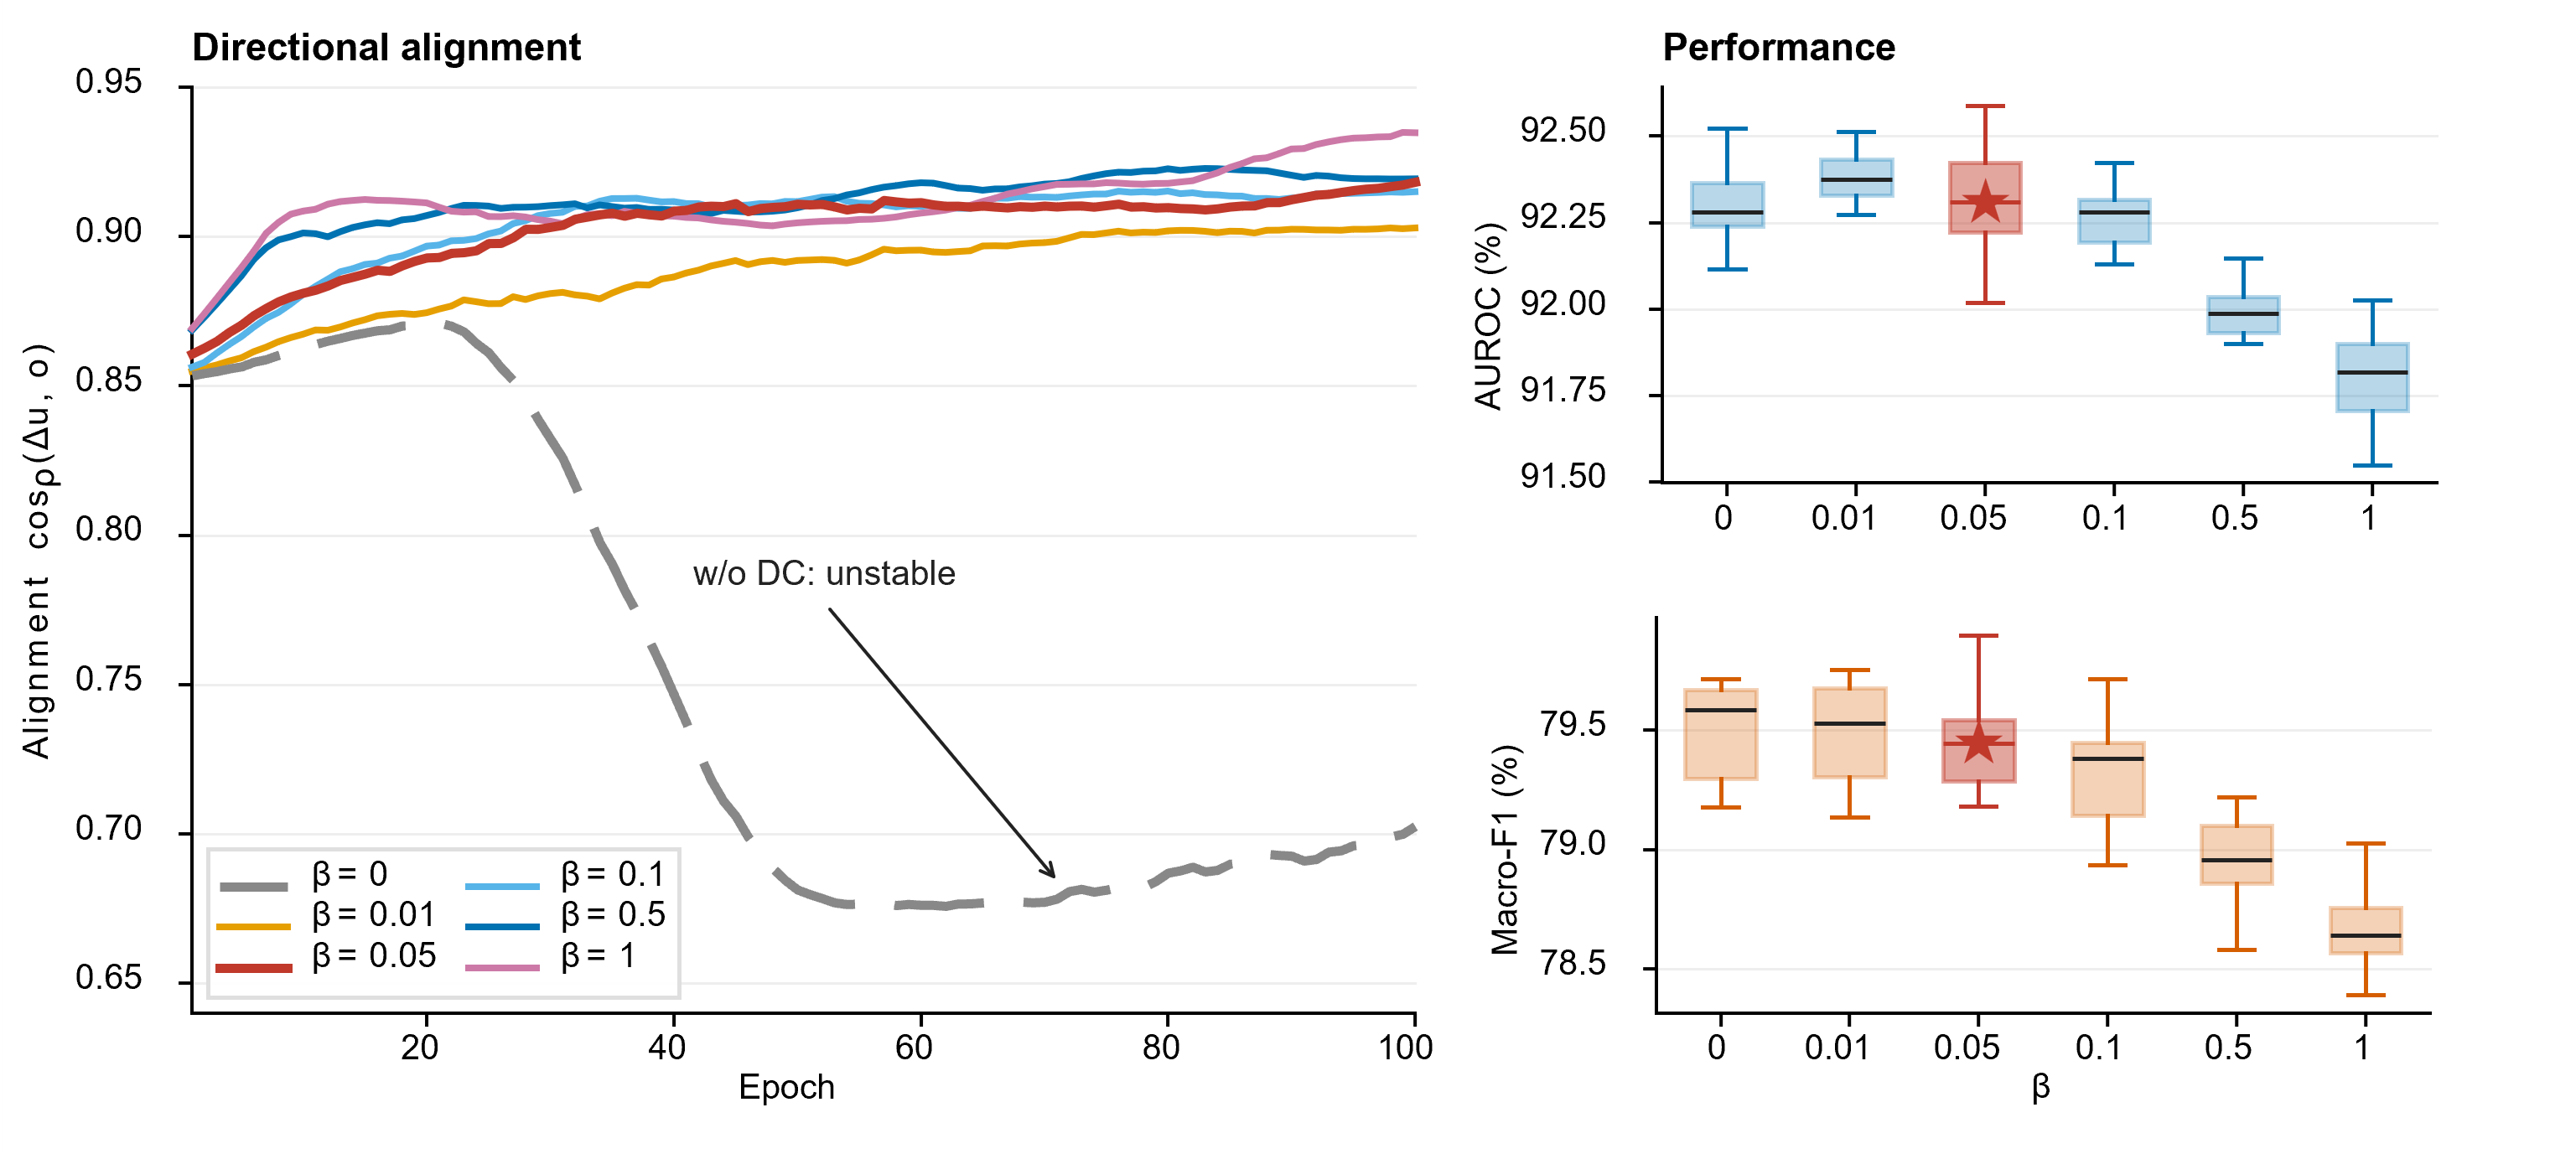
\includegraphics[width=\columnwidth]{fig_beta.png}
\caption{Directional alignment and predictive performance under different
values of $\beta$ on YelpChi. Left: evolution of the reliability-weighted
cosine agreement between the hidden class contrast and the estimated
orientation during training. Right: AUROC and Macro-F1 distributions over
ten runs. The selected setting $\beta=0.05$ is highlighted in red, with
stars marking its mean performance.}
\label{fig:beta}
\end{figure}

Figure~\ref{fig:beta} traces the evolution of directional agreement during
training. In the absence of directional consistency, the agreement improves
only in the early stage and then declines sharply, indicating that the
learned representation can drift away from the estimated orientation during
optimization. A small consistency weight largely suppresses this drift. At
the selected $\beta=0.05$, directional agreement reaches $92.3\%$, compared
with $69.1\%$ at $\beta=0$, while AUROC and Macro-F1 remain essentially
unchanged ($92.32\%/79.46\%$ versus $92.33\%/79.58\%$;
Table~\ref{tab:dc}). Increasing $\beta$ further provides little additional
gain in agreement and progressively reduces detection performance; at
$\beta=1$, agreement reaches $93.3\%$, whereas AUROC and Macro-F1 decrease
to $91.73\%$ and $78.57\%$. These results support directional consistency
as a mild regularizer that preserves the estimated orientation during
representation learning without imposing it too strongly on task-driven
adaptation.

\subsection{Sensitivity Analysis}
\label{sec:sensitivity}
We examine the sensitivity of SOAR through three hyperparameters acting at
different stages of the framework. The filter order $S$ determines the
resolution of the relation-wise spectral decomposition, $\lambda$ controls
the contribution of class-oriented residuals to prediction, and $\tau_n$
governs how labeled support is reflected in relation-level reliability.
These settings therefore probe the robustness of SOAR in spectral
resolution, residual strength, and reliability calibration.

\begin{figure}[!h]
\centering
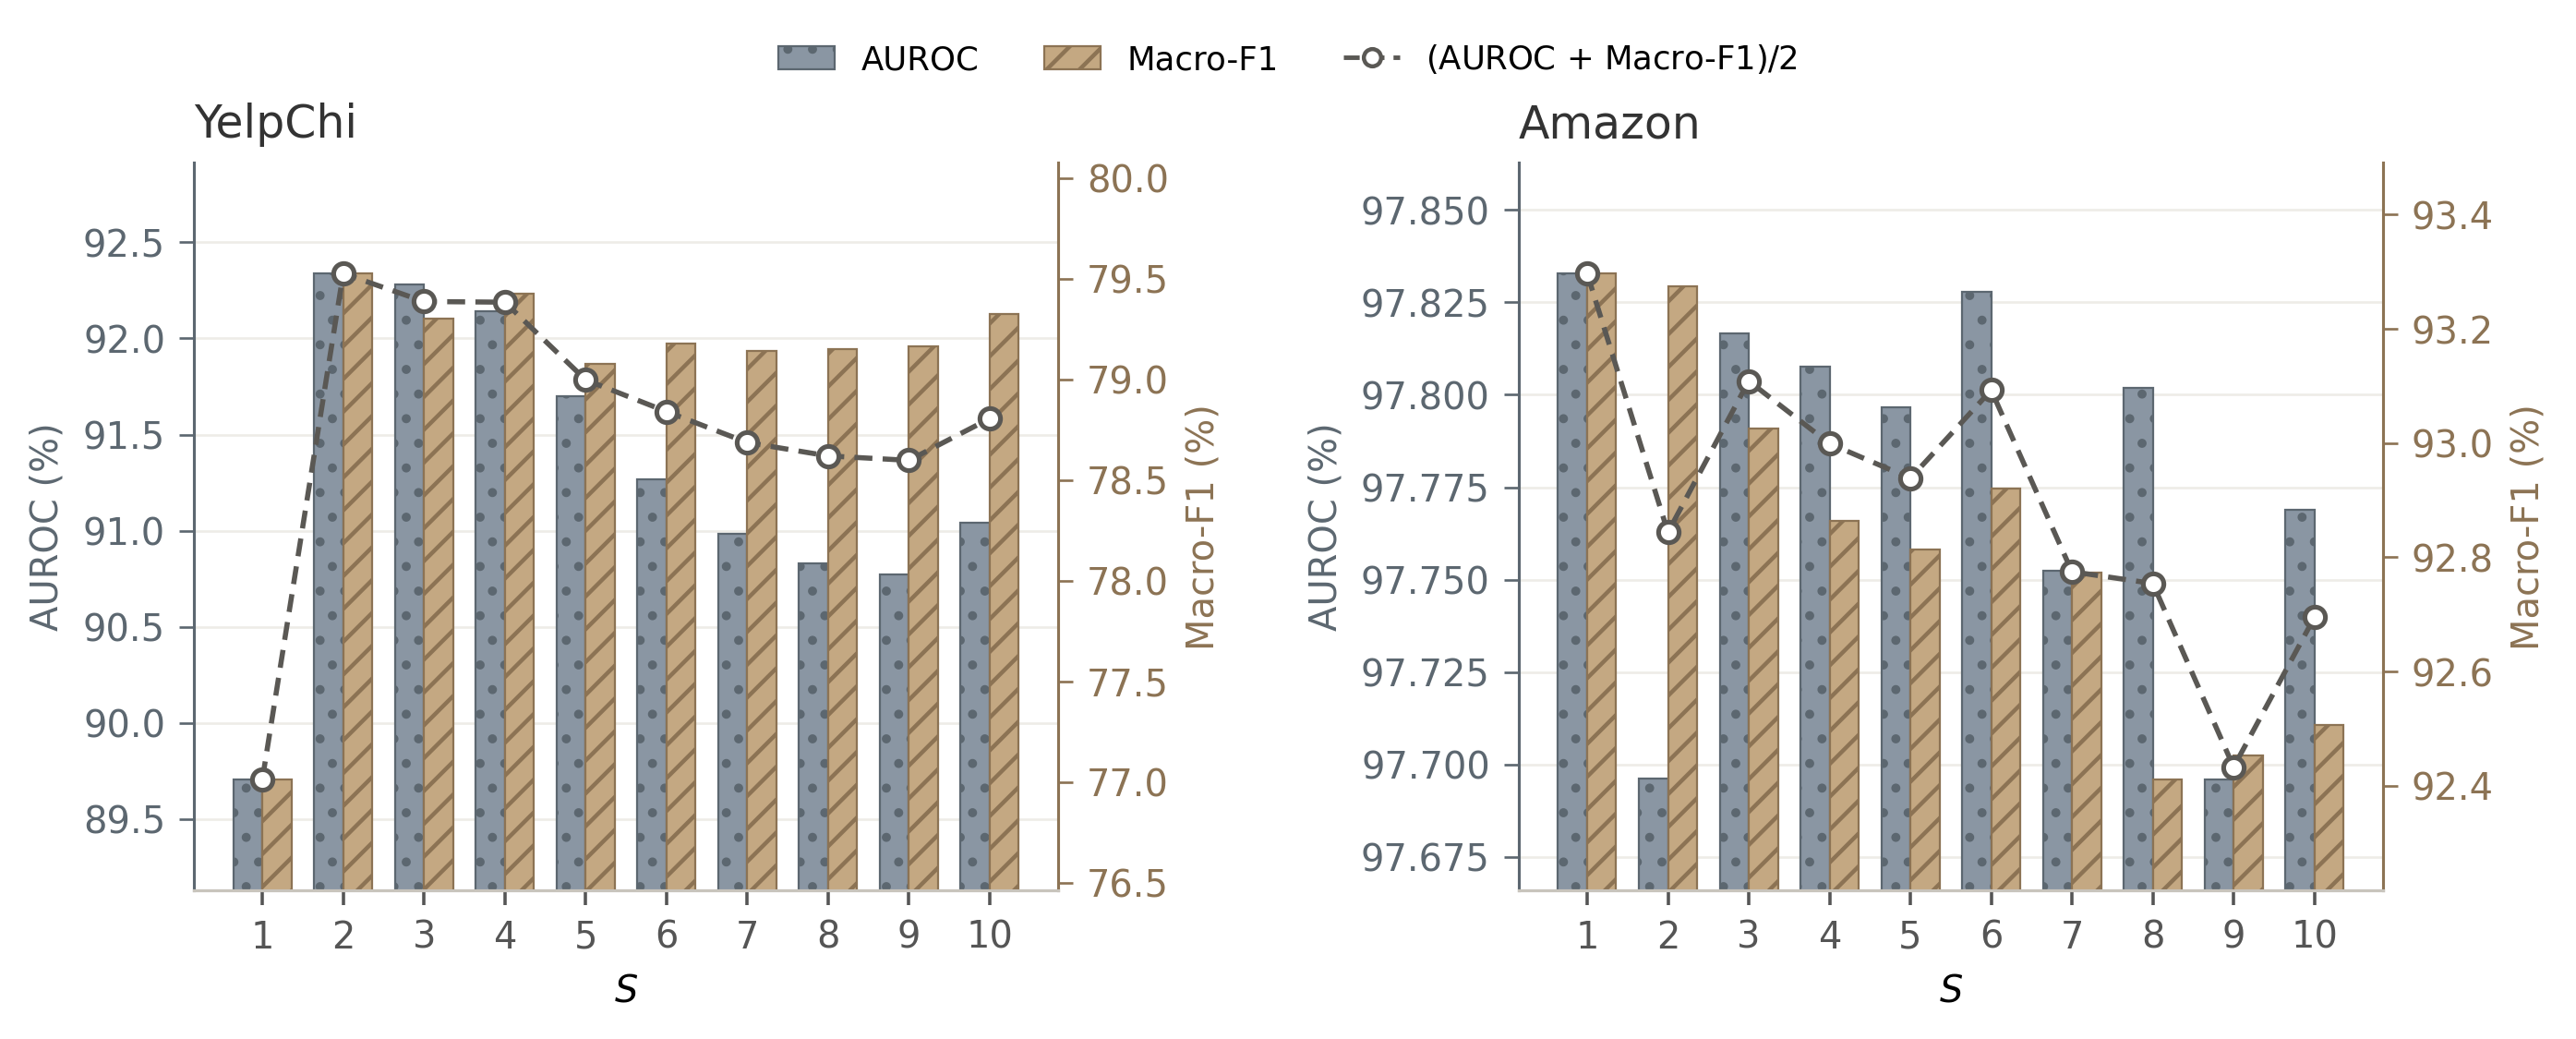
\includegraphics[width=\columnwidth]{fig_S_bars.png}
\caption{Sensitivity to the filter order $S$ on YelpChi and Amazon under
abundant supervision. The remaining hyperparameters are fixed to their main
experimental settings.}
\label{fig:sensitivity_s}
\end{figure}

\paragraph{Spectral Resolution} Varying $S$ changes the spectral partition itself. As shown in
Fig.~\ref{fig:sensitivity_s}, the coarsest decomposition is insufficient on
YelpChi, after which performance settles into a broad stable region. Amazon
shows only mild, non-monotonic variation across the tested orders. The
class-oriented spectral structure exploited by SOAR is therefore not tied to
a particular band partition once sufficient spectral resolution is available.

\begin{figure}[!h]
\centering
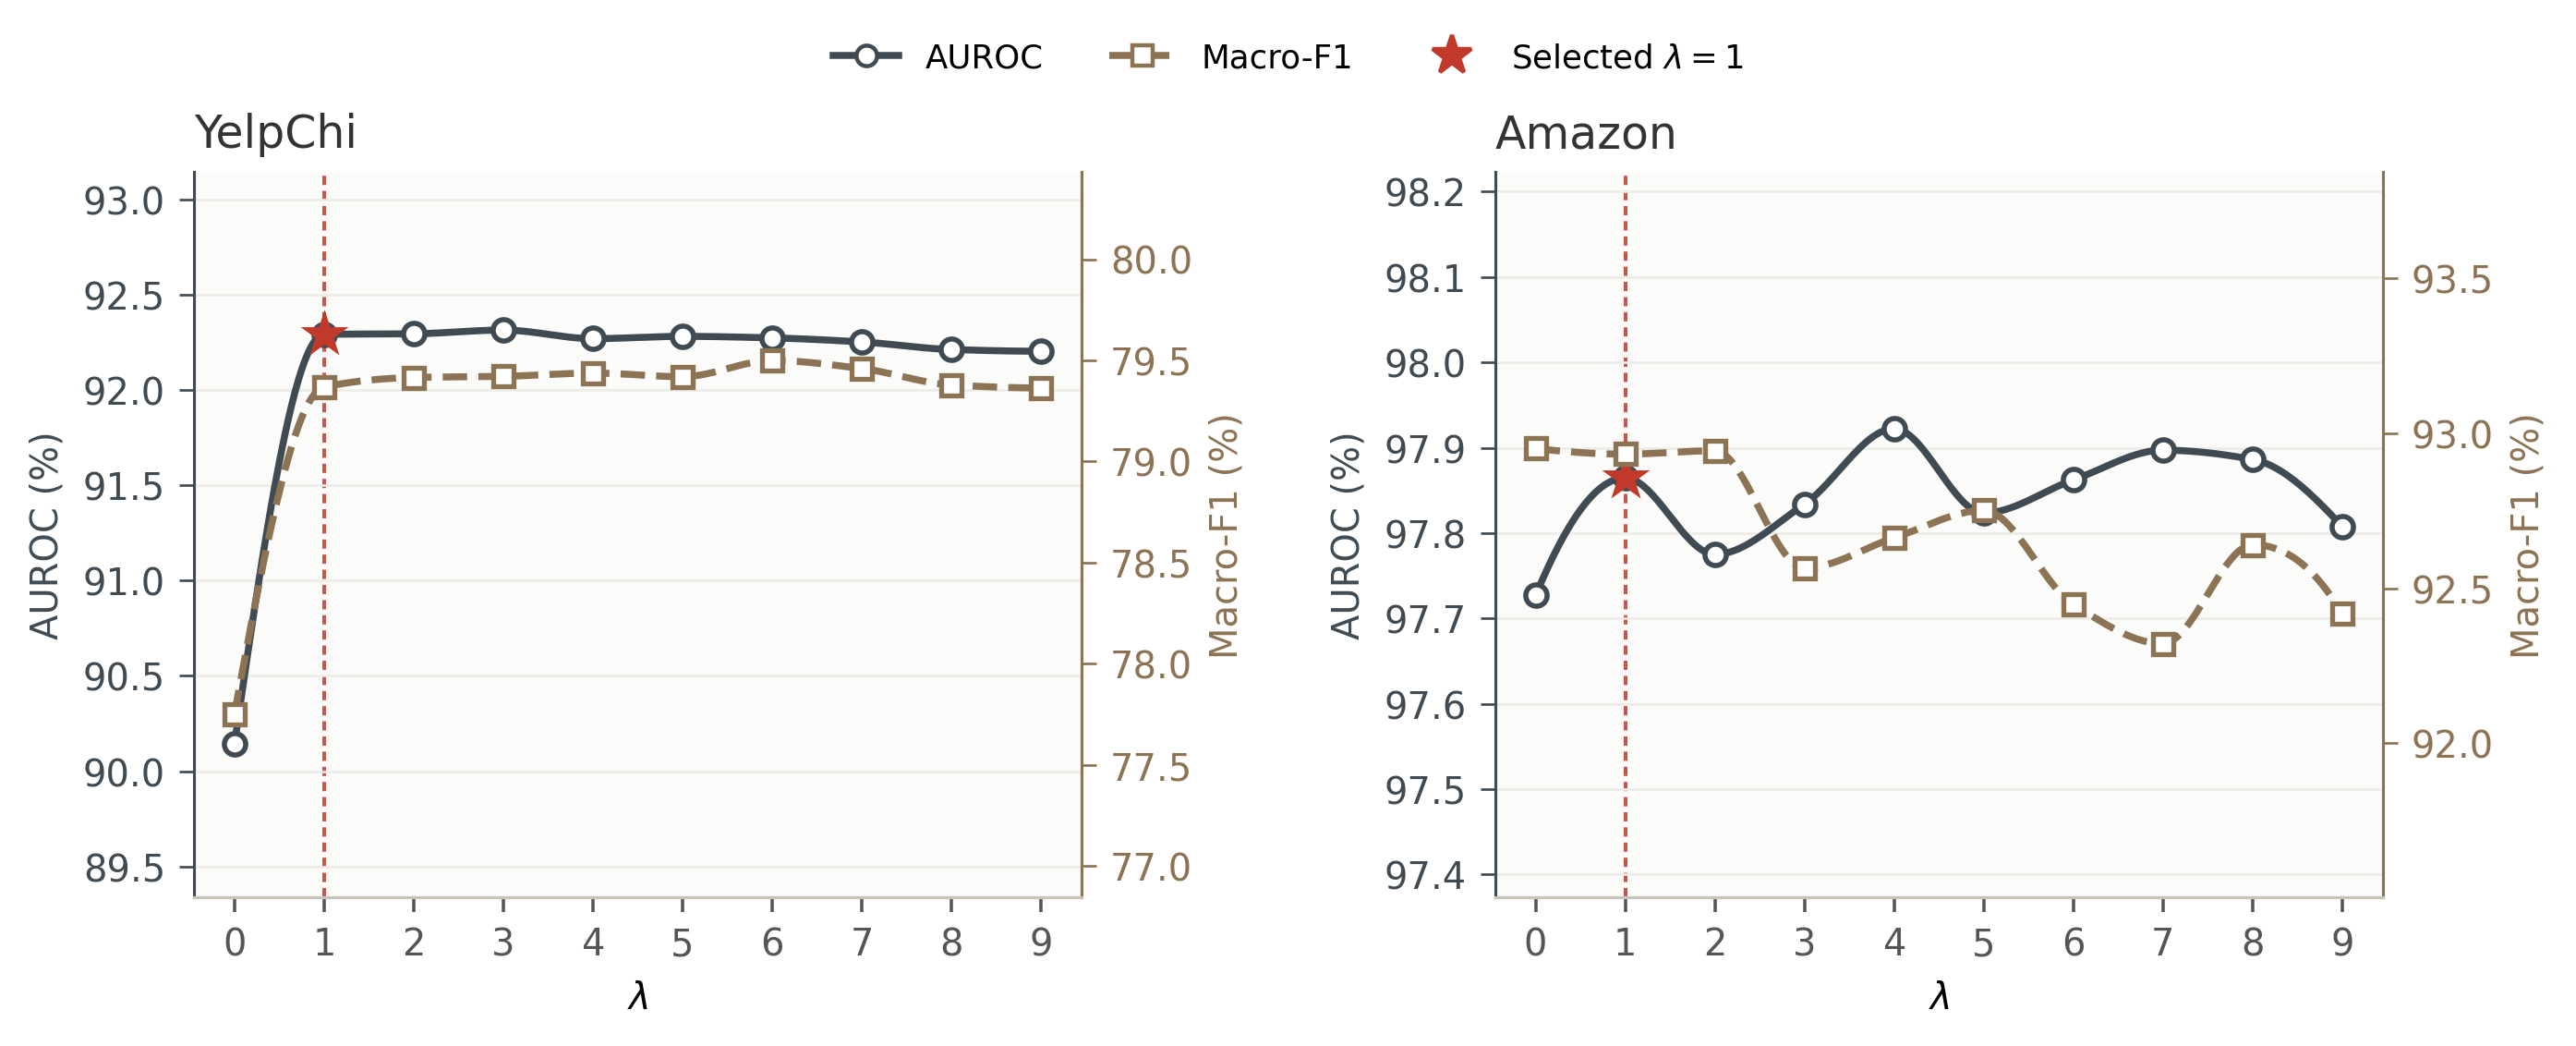
\includegraphics[width=\columnwidth]{fig_lambda.png}
\caption{Sensitivity to the signed-residual weight $\lambda$ on YelpChi and
Amazon under abundant supervision. The remaining hyperparameters are fixed
to their main experimental settings, and the marker indicates the selected
setting $\lambda=1$.}
\label{fig:sensitivity_lambda}
\end{figure}

\paragraph{Signed-Residual Strength} The sweep of $\lambda$ reveals a different pattern
(Fig.~\ref{fig:sensitivity_lambda}). On YelpChi, removing the signed
contribution from the readout leads to a clear degradation, whereas a broad
range of positive weights yields similar performance. Amazon varies little
throughout the tested range. Thus, the signed residual provides useful
class-oriented evidence, but its exact scale is not critical once it
complements the orientation-neutral path.

\begin{figure}[!h]
\centering
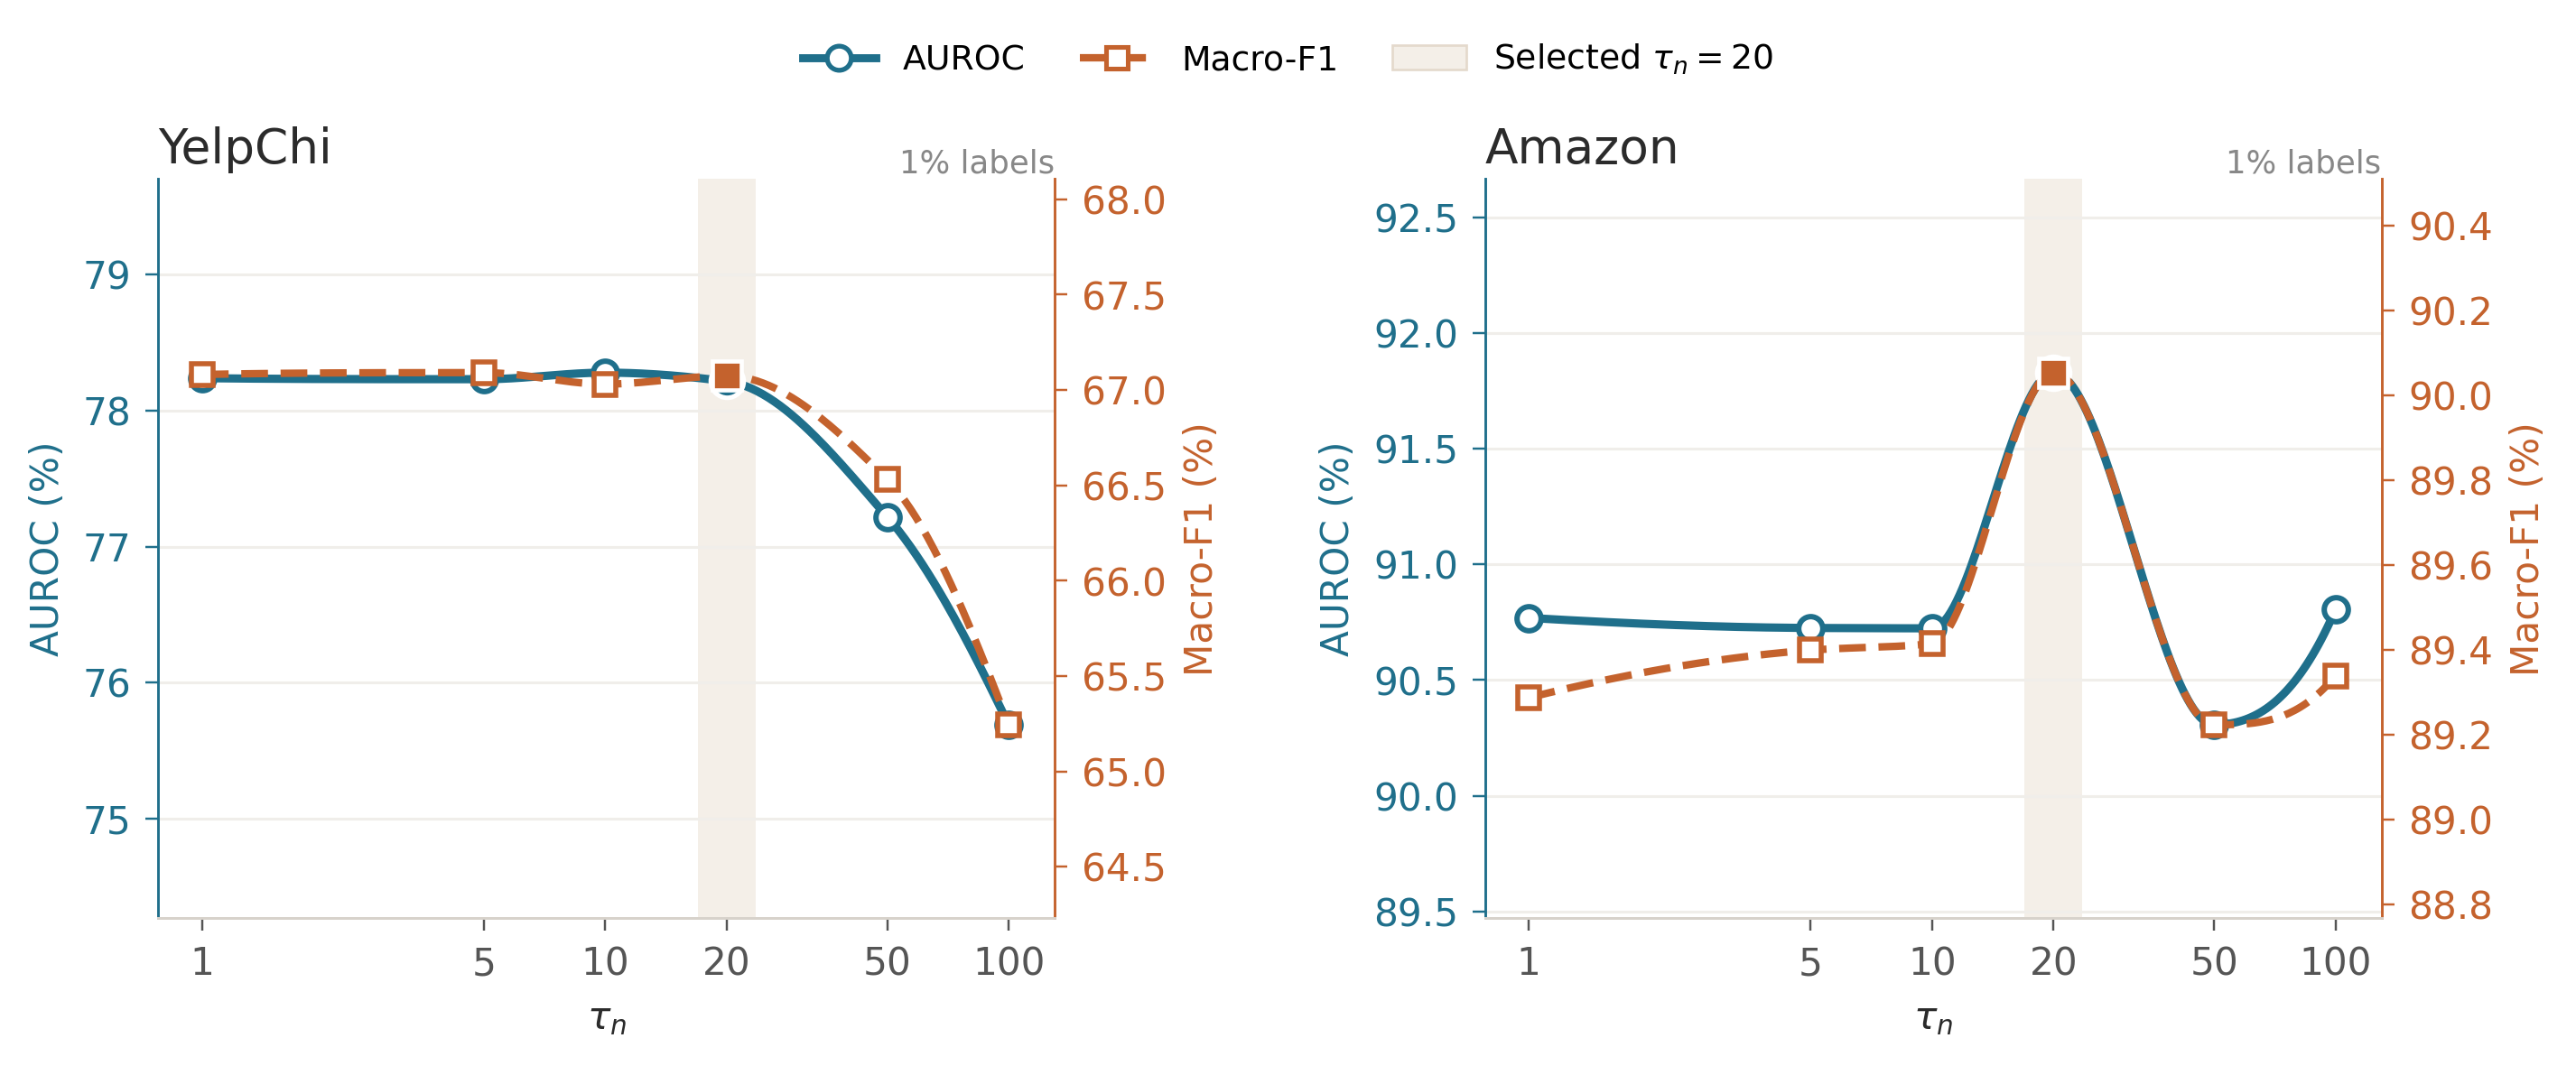
\includegraphics[width=\columnwidth]{fig_tau_scarce.png}
\caption{Sensitivity to the support saturation parameter $\tau_n$ on YelpChi
and Amazon under scarce supervision. The remaining hyperparameters are fixed
to their main experimental settings, and the marker indicates the selected
setting $\tau_n=20$.}
\label{fig:sensitivity_tau}
\end{figure}

\paragraph{Reliability Calibration} We examine $\tau_n$ under scarce supervision, where support calibration has a
more direct effect on relation-level reliability
(Fig.~\ref{fig:sensitivity_tau}). YelpChi remains stable across small to
moderate thresholds and degrades only when saturation becomes overly
conservative, whereas Amazon exhibits a clearer preference for an intermediate
setting. Together, the two datasets expose both sides of reliability
calibration: limited support should not saturate prematurely, but useful
orientation evidence should not remain excessively downweighted by an overly
large threshold.

\section{Conclusion}
\label{sec:conclusion}
This work studies class orientation as a distinct property of spectral
evidence in graph fraud detection. We find that relation--band responses with
comparable predictive relevance can favor opposite classes, while the
reliability of their estimated orientations can vary substantially across
relations when labeled support is limited. SOAR makes these properties
explicit by estimating relation--band class orientation together with
relation-level reliability, preserving class-oriented evidence through signed
residual learning while retaining orientation-neutral spectral information;
directional consistency further stabilizes the learned class contrast as the
representation evolves. Experiments on four real-world fraud graphs show
strong performance under both abundant and scarce supervision, while the
mechanism analyses support the complementary roles of orientation,
reliability calibration, and neutral spectral information. These results
highlight the importance of explicitly modeling class orientation and its
reliability in spectral graph fraud detection.

\bibliographystyle{IEEEtran}
\bibliography{references}
\end{document}
